%!TEX program = xelatex

\documentclass[cn,black,12pt,normal]{elegantnote}
\usepackage{float}
\usepackage{hyperref}
\usepackage{amsmath}
\usepackage{amsfonts}
\usepackage{amssymb}
\usepackage{siunitx}
\usepackage{fancyhdr}
\usepackage{newtxtext}
\PassOptionsToPackage{no-math}{fontspec}

\newcommand{\upcite}[1]{\textsuperscript{\textsuperscript{\cite{#1}}}}

\sisetup{mode=text}
\sisetup{range-phrase = \text{ \textasciitilde }}
\pagestyle{fancy}
\fancyhead[L]{School of Life Science, Tongji University}
\fancyhead[R]{实习报告}
\renewcommand{\headrulewidth}{1pt}

\title{\Huge 安徽金寨实习报告 \vspace*{300pt}}
\author{院(系):生命科学与技术学院\\专业:生命科学基地班\\学号:1951510\\学生姓名:姜文渊\\接受单位:安徽同科生物科技有限公司\\地址:金寨县现代产业园区金梧桐创业园A7楼\\指导老师:汪燕芳}
%\institute{School of Life Science, Tongji University}
%\version{1.00}
\date{2021年7月}

\begin{document}

\begin{titlepage}
    \centering

    %------------------------------------------------------------
    %    Top rules
    %------------------------------------------------------------

    %\rule{\textwidth}{1pt}   % The top horizontal rule
    \vspace{0.2\textheight}  % Whitespace between top horizontal rule and title
    

    %------------------------------------------------------------
    %    Title
    %------------------------------------------------------------
    
\includegraphics[width=0.5\textwidth]{image/tongji-whole-logo.eps}

    \vspace{0.02\textheight}

    {\Huge 安徽金寨实习报告}

    

    \vspace{0.25\textheight}  % Whitespace between the short horizontal rule and author

    %------------------------------------------------------------
    %    Author
    %------------------------------------------------------------

    \begin{flushleft}
        \hspace{0.3\textwidth}
        院(系):生命科学与技术学院

        \hspace{0.3\textwidth}
        专业:生命科学基地班

        \hspace{0.3\textwidth}
        学号:1951510

        \hspace{0.3\textwidth}
        学生姓名:姜文渊

        \hspace{0.3\textwidth}
        接受单位:安徽同科生物科技有限公司

        \hspace{0.3\textwidth}
        地址:金寨县现代产业园区金梧桐创业园A7楼

        \hspace{0.3\textwidth}
        指导老师:汪燕芳
    \end{flushleft}
    \vspace{0.05\textheight}
    %{院(系):生命科学与技术学院\\专业:生命科学基地班\\学号:1951510\\学生姓名:姜文渊\\接受单位:安徽同科生物科技有限公司\\地址:金寨县现代产业园区金梧桐创业园A7楼\\指导老师:汪燕芳}
    \begin{flushleft}
        {\scriptsize 关于实习报告中不详尽的内容:实习报告中,笔者希望做到尽可能详尽地记录实习的内容,但是实习过程中,诸多内容涉及到接受单位的\textbf{受控文件},因而不得已进行模糊化的处理(例如设备的使用方法,生产检测过程中具体体系配置的用量细节等)。实习中,涉及到受控文件等部分,如果还有处理不当等部分,望有关人员指出并联系笔者改正。}
    \end{flushleft}
    \vfill  % Whitespace between author and date
    
    {\large 2021年7月}
    %\vspace{0.1\textheight}  % Whitespace between date and bottom horizontal rule

    %------------------------------------------------------------
    %    Bottom rules
    %------------------------------------------------------------

    %\rule{\textwidth}{1pt}  % The bottom horizontal rule

\end{titlepage}

%\maketitle
\newpage
\tableofcontents
\newpage

\section{实习目的}

本次实习,企业将组织两批次体外诊断试剂的生产活动,实习生分成两组,分批次参与参与到试剂生产、分装、半成品检验、贴签包装、成品检验等实际作业活动中去。通过理论知识培训及不同岗位上的实际操作了解以下内容。

\begin{itemize}
    \item 企业组织模式
        \subitem 文件管理
        \subitem 采购过程管理
        \subitem 仓储物流管理
        \subitem 体系运行管理
        \subitem 销售过程控制
    \item 质量管理体系模式
        \subitem 行业法规
        \subitem 产品质量管理相关知识
    \item 产品生产及检验流程
        \subitem 产品相关知识
        \subitem 体外诊断试剂生产、检验过程操作
        \subitem 体外诊断试剂生产、检验过程注意事项
    \item 各个岗位职责
\end{itemize}

\section{实习单位简介}

同科生物成立于2007年,是一家集研发、生产、销售和技术服务于一体专注于生命医学和生物技术领域的高新技术企业,其主要产品为各类临床分子诊断试剂盒(如人乳头瘤病毒核酸分型检测试剂盒等)以及各类重要生物制剂(PCR Mixes等)、仪器(TK6000 PCR仪),此外,同科生物也提供细胞实验相关技术服务(细胞增殖试验、细胞周期检测等)。

该公司拥有三类体外试剂生产中心、仪器生产中心、研发质检实验室等、厂房和实验面积达8000多平米,仪器设备设施先进齐全(包括定量PCR仪、生物安全柜、超净工作台、核酸蛋白测定仪、高压细胞破碎仪、FPLC等系列高端精密仪器设备)

其经营范围为:生物科技、农业科技、化工产品领域内的技术研发、技术服务、技术转让、技术咨询;从事生物试剂、仪器设备、医疗器械(一类、二类、三类)、化工产品(不含危险化学品)的生产、销售及进出口业务。

本次实习的接受单位为安徽同科生物科技有限公司,其位于安徽省金寨县金梧桐创业产业园 A7 楼。
该单位为同科生物的诊断试剂产品化中心,其主要职能为进行各类临床分子诊断试剂盒的生产。
安徽同科生物科技有限公司所在的A7楼为一四层的建筑,其中,生产车间位于一楼,而检验实验室等位于二楼。


\section{实习日程简介}

本次实习的日程安排主要分为以下几大块:
\begin{itemize}
    \item 理论培训
    \item 生产过程实践
    \item 检验过程实践
    \item 参观与交流学习
\end{itemize}

其中,理论培训集中在实习的前两天上午;生产过程实践为实习的主要内容之一,会占用数个全天的时间;检验过程实践主要在生产开始前以及半成品和成品完成后进行,占用数个半天时间;其余的时间用于安排参观与交流学习。

具体的实习时间参考实习手册中的安排表,简要列举如下。

\begin{enumerate}
    \item 7月21日:通勤;欢迎会
    \item 7月22日:理论培训;原料检验
    \item 7月23日:清场;理论培训
    \item 7月26日:产品生产;环境检测
    \item 7月27日:产品生产;产品组装
    \item 7月28日:成品检验
    \item 7月29日:成品检验;实习总结
    \item 7月30日:返程
\end{enumerate}

\section{理论培训}

\subsection{行业法规培训及体系运行控制管理}
行业法规培训及体系运行控制管理的培训于7月22日上午进行。

本次培训涉及的内容包含了医疗器械以及体外诊断试剂行业的一些基本概念,相关法律法规的概况,以及该行业的发展现状等。该培训介绍范围较广,因而涉及的细节不多。考虑到笔者等的知识体系基础,该培训补足了笔者对知识体系的一些空白,也让笔者对于行业法规等内容的复杂程度有了一个感性的认识。对于更加深入的内容,笔者希望在以后的学习或者实践中有机会做更多更加深入且详细等了解。

\subsubsection{医疗器械以及体外诊断试剂行业的基本概念}

\paragraph{医疗器械的定义}
医疗器械是指直接或者间接用于人体的仪器、设备、器具、体外诊断试剂及校准物、材料以及其他类似或者相关的物品,包括所需要的计算机软件;其效用主要通过物理等方式获得,不是通过药理学、免疫学或者代谢的方式获得,或者虽然有这些方式参与但是只起辅助作用;其目的是:
\begin{itemize}
    \item 疾病的诊断、预防、监护、治疗或者缓解;
    \item 损伤的诊断、监护、治疗、缓解或者功能补偿;
    \item 生理结构或者生理过程的检验、替代、调节或者支持;
    \item 生命的支持或者维持;
    \item 妊娠控制;
    \item 通过对来自人体样本进行检查的方式来提供医疗信息。
\end{itemize}
\textit{来源:医疗器械监督管理条例(国令第739号)}

\paragraph{医疗器械的分类}
医疗器械的分类方式较为多样,可以有如下分类。
\begin{itemize}
    \item 根据结构特征的不同,分为无源医疗器械和有源医疗器械。
    \item 根据是否接触人体,分为接触人体器械和非接触人体器械。根据不同的结构特征和是否接触人体,医疗器械的使用形式包括:
        \subitem 无源接触人体器械:液体输送器械、改变血液体液器械、医用敷料、侵入器械、重复使用手术器械、植入器械、避孕和计划生育器械、其他无源接触人体器械。
        \subitem 无源非接触人体器械:护理器械、医疗器械清洗消毒器械、其他无源非接触人体器械。
        \subitem 有源接触人体器械:能量治疗器械、诊断监护器械、液体输送器械、电离辐射器械、植入器械、其他有源接触人体器械。
        \subitem 有源非接触人体器械:临床检验仪器设备、独立软件、医疗器械消毒灭菌设备、其他有源非接触人体器械。
    \item 根据不同的结构特征、是否接触人体以及使用形式,医疗器械的使用状态或者其产生的影响包括以下情形:
        \subitem 无源接触人体器械:根据使用时限分为暂时使用、短期使用、长期使用;接触人体的部位分为皮肤或腔道(口)、创伤或组织、血液循环系统或中枢神经系统。
        \subitem 无源非接触人体器械:根据对医疗效果的影响程度分为基本不影响、轻微影响、重要影响。
        \subitem 有源接触人体器械:根据失控后可能造成的损伤程度分为轻微损伤、中度损伤、严重损伤。
        \subitem 有源非接触人体器械:根据对医疗效果的影响程度分为基本不影响、轻微影响、重要影响。
\end{itemize}
此外,医疗器械\textbf{按照风险程度由低到高},管理类别依次分为\textbf{第一类、第二类和第三类}。医疗器械风险程度,应当根据医疗器械的预期目的,通过结构特征、使用形式、使用状态、是否接触人体等因素综合判定。

\textit{来源:《医疗器械分类规则》(国家食品药品监督管理总局令第15号)}


\paragraph{体外诊断试剂定义}
指按医疗器械管理的体外诊断试剂,包括在疾病的预测、预防、诊断、治疗监测、预后观察和健康状态评价的过程中,用于人体样本体外检测的试剂、试剂盒、校准品、质控品等产品。可以单独使用,也可以与仪器、器具、设备或者系统组合使用。\textbf{按照药品管理的用于血源筛查的体外诊断试剂和采用放射性核素标记的体外诊断试剂,不属于本办法管理范围。}

\textit{来源:《体外诊断试剂注册管理办法》(国家食品药品监督管理总局令第5号)}



\subsubsection{医疗器械以及体外诊断试剂行业的相关法律法规}
在该领域,常见的法规大致分为以下几类。
\begin{itemize}
    \item 法律行政法规 (例如:《医疗器械监督管理条例》(国务院令第650号))
    \item 部门规章(例如:《体外诊断试剂注册管理办法》(国家食品药品监督管理总局令第5号))
    \item 工作文件(例如:《总局办公厅关于医疗器械产品技术要求有关问题的通知》(食药监办械管〔2016〕22号))
    \item 征求意见(例如:关于征求相关医疗器械注册事项办理程序意见的函(2015.09.28))
    \item 政策解读(例如:《医疗器械临床试验质量管理规范》解读 (2016.03.23))
\end{itemize}

医疗器械监督管理条例配套法规涵盖了医疗器械分类管理、创新管理、标准管理、诚信管理、注册管理、临床试验管理、临床试验机构管理、临床试验审批管理、生产管理、供应商管理、产品技术要求管理、命名管理、器械说明书标签管理、委托生产管理、经营管理、使用管理、进出口管理、广告管理、不良事件管理等多个方面的内容,实习报告里甚至无法逐一列举相关法规的名称,由此可见相关法规及规范的细致程度。

\subsubsection{医疗器械以及体外诊断试剂行业的的发展现状}
近年来,随着全球居民生活水平的提高和医疗保健意识的增强,医疗器械产品需求持续增长。2020年全球医疗器械行业市场规模为4774亿美元,同比增长5.63\%,预计到2024年全球医疗器械行业规模将达接近6000亿美元,2017-2024年复合增长率为5.6\%,行业有望保持稳定增长。(\textit{来源:Evaluate MedTech})

国内医疗器械市场将保持20\%的增速发展,未来市场空间巨大。我国医疗器械和药品人均消费额的比例仅为0.35:1,远低于0.7:1的全球平均水平,更低于欧美发达国家0.98:1的水平。因为消费群体庞大、健康需求不断增加以及政府的积极支持,我国医疗器械市场发展空间极为广阔。截至2020年,中国医疗器械市场规模约为7341亿元,同比增长18.3\%,接近全球医疗器械增速的4倍,维持在较高的增长水平,中国已经成为仅次于美国的全球第二大医疗器械市场。预计未来5年,器械领域市场规模年均复合增长率约为14\%,至2023年将突破万亿。

从我国医疗器械市场的产品结构看,影像诊断设备占据最大的市场份额;其次是体外诊断,占据14\%的市场份额;低值耗材占据13\%的市场份额;剩余的市场份额被心血管、骨科及其他类器械所占据。随着国家鼓励创新医疗器械研发生产、医疗器械国产化及进口替代政策的实施,我国自主创新的医疗器械将会加速涌现,产品实现中低端市场向高端市场的不断突破。以\textbf{体外诊断试剂}、骨科医疗器械、心血管医疗器械、医学影像设备和高值耗材为主的细分领域成为国家鼓励发展和行业投资重点。

\subsection{本次生产产品介绍}
本次生产产品介绍的培训于7月22日上午进行。

\subsubsection{产品介绍及生产培训} 本次生产一共涉及该公司的两种产品:
\begin{enumerate}
    \item 人乳头瘤病毒(15个型)核酸分型检测试剂盒(PCR多色荧光法)
    \item 人乳头瘤病毒(27个型)核酸分型检测试剂盒(PCR多色荧光法)
\end{enumerate}

这两种产品的原理大致相同,都是利用rtPCR多色荧光法,即TaqMan探针,对提取的DNA进行扩增和检测。rtPCR中,共利用四种通道(FAM, JOE/HEX, ROX, CY5),检测多种HPV和HBB基因(HBB为内参)。反应体系中主要为dNTP,引物,探针,Taq酶,UNG酶,以及适当的缓冲溶液。

\paragraph{产品的构成} 包括DNA提取液、各种反应预混合液,酶混合液,阴性对照和阳性对照。

\paragraph{关于rtPCR/qPCR} 聚合酶链式反应 (PCR) 可对特定核苷酸片断进行指数级的扩增 。在扩增反应结束之后,我们可以通过凝胶电泳的方法对扩增产物进行定性的分析,也可以通过 放射性核素掺入标记后的光密度扫描来进行定量的分析。无论定性还是定量分析,分析的都是 PCR 终产物。但是在许多情况下,我们所感兴趣的是未经 PCR 信号放大之前的起始模板量。例如我们想知道某一转基因动植物转基因的拷贝数或者某一特定基因在特定组织中的表达量。在这种需求下荧光定量 PCR 技术应运而生。所谓的实时荧光定量 PCR 就是 通过对 PCR 扩增反应中每一个循环产物荧光信号的实时检测从而实现对起始模板定量及定性的分析。在实时荧光定量 PCR 反应中,引入了一种荧光化学物质,随着 PCR 反应的进行, PCR 反应产物不断累计,荧光信号强度也等比例增加。每经过一个循环,收集一个荧光强度信号,这样我们就可以通过荧光强度变化监测产物量的变化,从而得到一条荧光扩增曲线图。一般而言,荧光扩增曲线扩增曲线可以分成三个阶段:荧光背景信号阶段 , 荧光信号指数扩增阶段和平台期。在荧光背景信号阶段,扩增的荧光信号被荧光背景信号所掩盖,我们无法判断产物量的变化。而在平台期,扩增产物已不再呈指数级的增加。 PCR 的终产物量与起始模板量之间没有线性关系,所以根据最终的 PCR 产物量不能计算出起始 DNA 拷贝数。只有在荧光信号指数扩增阶段, PCR 产物量的对数值与起始模板量之间存在线性关系,我们可以选择在这个阶段进行定量分析。

\textbf{值得注意的是,该产品的生产流程中,关键步骤为混合与分装,而更加有价值的探针的序列,则为公司的机密,一般不会外泄。}

\subsubsection{产品生产中的基本概念}

\paragraph{生产的要素} 包括人员、基础设施、材料、工艺、生产环境和质量控制。通过这些要素的相互作用,企业可以生产出产品或者提供一些服务。

\paragraph{生产涉及的主要内容} 包括生产的工艺配方、标准操作流程、物料平衡、批生产记录、防止污染和混淆的措施、清场措施、生产设备的管理。

\paragraph{生产过程} 在本次实习生产的产品的生产中,主要包括生产前准备,试剂称量,试剂配置,试剂分装,试剂灯检。本次生产不包括特殊过程(\textbf{特殊过程是指某些加工质量不易或不能通过其后的检验或试验而得到充分验证的过程})。

生产过程的具体细节详见下面的生产过程实践部分。

\subsection{产品检验培训}
产品检验培的培训于7月22日上午进行。

\subsubsection{产品检验的基本概念}

\paragraph{质量的定义} 客体的一组固有特性满足要求的程度。

\paragraph{公司质量控制的两大部门} 监督部门和检验部门。其中,监督部门负责建立质量控制规范,构建相关的框架;而检验部门则负责对于特定的对象进行质量检验。

\paragraph{检验的分类} 按照检验所处在生产过程中的流程,可以分为:进货检验(IQC),过程检验(IPQC),最终检验(FQC)以及出货检验(OQC)

\paragraph{各过程中多次检验的目的} 可以在生产前期监测异常,从而尽早停止生产或进行补救,继而减少公司的损失。此外,各个过程中进行多次检验也增加了生产过程的可追溯性,有助于改进生产工艺或流程。

\paragraph{检验的抽样方法} 包括全数检验与抽样检验。全数检验一般用于:重要的、关键的和贵重的制品;对以后工序加工有决定性影响的项目;质量严重不匀的工序和制品;不能互换的装配件;批量小,不必抽样检验的产品。

\subsubsection{本次实习涉及到的检验}
\begin{itemize}
    \item 纯化水检验
    \item 洁净环境检验
    \item 物资验收检验
    \item 产品检验
\end{itemize}

\subsection{质量管理体系文件控制培训}

\subsubsection{文件管理的目的与意义} 第一,保证了企业所有生产活动都是有资料可参考,有利于生产人员更方便地掌握生产方法及相关操作;第二,保证了企业所有生产活动都是有文字记录的,有利于监督人员更好地进行监督,当问题出现时,更容易发现问题;第三,各类文件是企业本身的要求,是国家规范化的结果,是人民财产安全的一道防线。

\subsubsection{文件管理涉及的标准及法规}
\begin{itemize}
    \item GBT 19000-2016
    \item GBT 19001-2016
    \item YYT 0287-2017
    \item 医疗器械生态质量管理规范
    \item 医疗器械生产质量管理规范
    \item 体外诊断试剂现场检查指导原则
\end{itemize}

\subsubsection{文件的分类} 企业文件一般分为三类——外来文件(包括国家标准,行业法规)、产品文件(包括产品信息,产品生产流程)、管理文件(包括体系监督,生产管理)。在该企业中,文件又被分为5级(1级为最高级),较低级文件是较高级文件的细化。例如,2级文件为生产程序文件,而对应的3级文件则是作业指导性文件(SOP),对应的4级文件为空白的记录表。各级别文件及其描述如下所示。

\begin{itemize}
    \item 一级文件:质量手册、质量方针、质量目标
    \item 二级文件:程序文件
    \item 三级文件:质量管理文件、作业指导性文件
    \item 四级文件:空白制式表格
    \item 五级文件:质量记录
\end{itemize}

为方便使用与管理,文件在公司内的类别通常以文件类别代码表示,例如一级文件中的质量手册用代码QM表示。分类的代码也被用在文件等编码中。

\subsubsection{文件的编码} 文件的数量庞大,在企业内部需要有统一的专门的编号,有利于文件分类和查找。通常意义上的文件受控于专门的文件管理部门,从规章制度到使用章程,从评估体系到质量保证,实时记录人、事、地、时,原始的记录是种清洗保留,以便于日后筛查。

下面举文件编码的例子一则,说明该公司文件编码的大致规则。现有一份一级文件,编码如下:\texttt{TK/QM-001B/0}。其中,TK代表该公司的名称,斜杠后的QM代表文件类别,横杆后的编号为流水号,流水号后的大写字母为版本号,版本号后斜杠,其后的数字代表修改状态。一级文件编码方式简要表示为:\texttt{TK/文件类别-流水号+版本号/修改状态}。其余各级各类文件编码方式类似。

\subsubsection{文件控制过程}

该公司的文件控制流程大致如下图所示。

\begin{figure}[H]
    \centering
    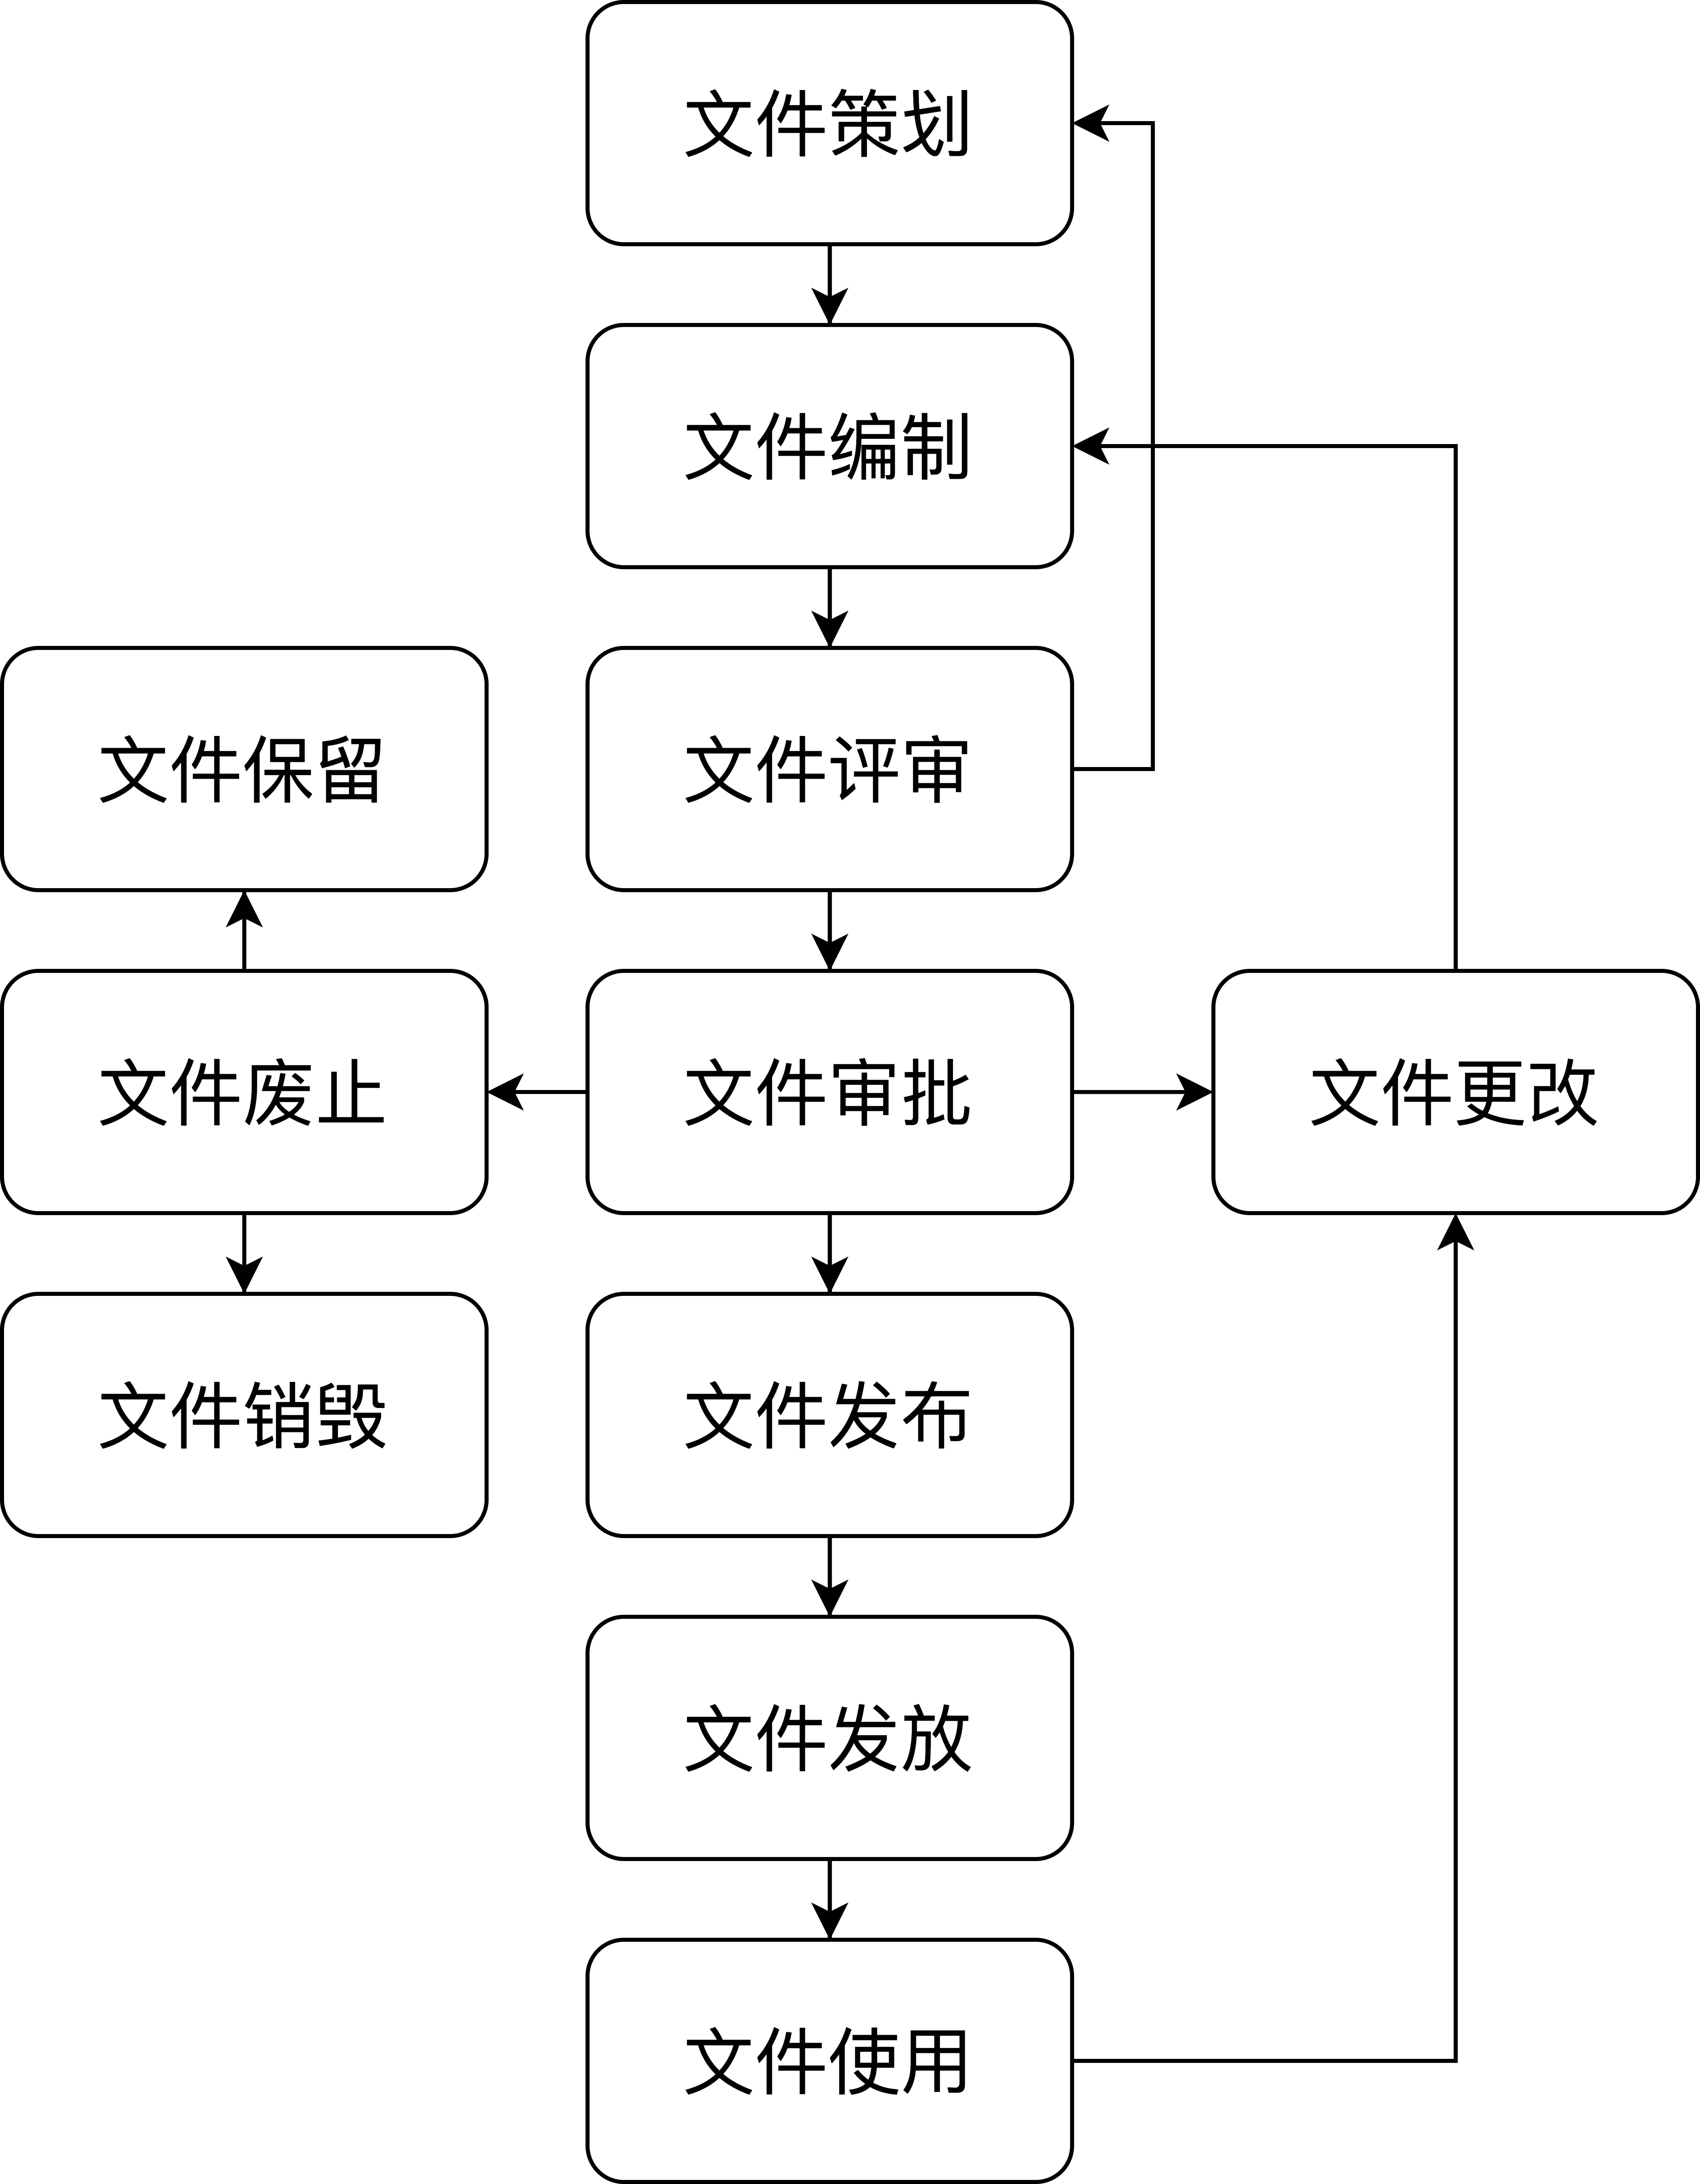
\includegraphics[width=0.7\textwidth]{image/DocumentControl.png}
    \caption{文件控制过程简图}
    \label{FC}
\end{figure}

\subsection{生产车间及实验室培训}
生产车间及实验室培训于7月23日下午进行。

\subsubsection{洁净车间基本知识}
洁净室及相关受控环境将空气悬浮粒子控制在适当的水平,以便完成对污染敏感的活动,航空航天、微电子、制药、医疗器械、食品、医疗卫生等行业的产品和工艺受益于对悬浮污染物的控制。

\paragraph{洁净室 cleanroom} 空气悬浮粒子浓度受控的房间,其建造和使用方式使房间内进人的、产生的、滞留的粒子最少,房间内温度、湿度、压力等其他相关参数按要求受控。

\paragraph{洁净区 clean zone} 空气悬浮粒子浓度受控的专用空间,其建造和使用方式使区内进人的、产生的、滞留的粒子最少,区内温度、湿度、压力等其他相关参数按要求受控,注,洁净区可以是开放的或封闭的,可在也可不在洁净室内。

\paragraph{设施 installation} 所有相关构筑物、空气处理系统以及服务、公用系统的洁净室,建一个或数个这样的洁净区。

\paragraph{洁净度等级 classification} 洁净度等级classification 以ISO N级表示的、洁净室或清净区内按空气悬浮粒子浓度划分的洁净度水平(或规定、确定该水平的过程)。洁净度等级代表关注粒径粒子的最大允许浓度(表示为每立方米空气中的粒子个数)。

\subsubsection{洁净车间相关法律法规}

洁净车间的设计,建设,运行等,均有相关法律法规为依据,下面简要列举一些。
\begin{itemize}
    \item 《洁净厂房设计规范》(GB50073)
    \item 《医疗器械生产质量管理规范》
    \item 《关于发布医疗器械生产质量管理规范附录体外诊断试剂的公告》
    \item YY 0033-2000 无菌医疗器具生产管理规范
    \item YY/T 0567.1-2013 医疗产品的无菌加工
    \item 《体外诊断试剂生产实施细则(试行)》
\end{itemize}

\subsubsection{维持洁净车间运行的主要设备}

\paragraph{空调净化系统} 为了使洁净室内保持所需要的温度湿度、风速、压力和洁净度等参数,最常用的方法是向室内不断送入一定量经过处理的空气,以消除洁净室内外各种热湿干扰及尘埃污染。为获得送入洁净室具有一定状态的空气,就需要一整套设备对空气进行处理,并不断送入室内,又不断从室内排出一部分来,这一整套设备就构成了洁净空调系统。

集中式洁净空调系统。在系统内单个或多个洁净室所需的净化空调设备都集中在机房内,用送风管道将洁净空气配给各个洁净室。主要有如下特点:

\begin{enumerate}
    \item 在机房内对空气集中处理,进而送进各个洁净室。
    \item 由于设备集中于机房,对噪声和振动较容易处理。
    \item 一个系统控制多个洁净室,要求各洁净室同时使用系数高。
    \item 集中处理后的洁净空气送入各洁净室,以不同的换气次数和气流形式来实现各洁净室内不同的洁净度。
\end{enumerate}

\paragraph{纯化水系统} 反渗透纯水系统是通过反渗透膜法来制取纯水的装置。反渗透是一种利用高分子膜进行物质分离的过程,可以从水中除去 90\% 以上的溶解盐类及 99\% 以上的胶体。
包括:原水、原水箱、原水泵、多介质过滤器、活性碳过滤器、软化器、一级精密过滤器、一级反渗透、混合离子交换器、臭氧发生器、纯水箱、紫外杀菌器、纯水泵、用水点。

电去离子交换系统(EDI)的纯化水设备是一种离子交换系统,这种离子交换系统使用一个混合树脂床,采用选择性的渗透膜以及充电器,以保证纯化水设备的连续进行和树脂的连续再生。

纯化水设备处理工艺为,原水首先进入树脂段,当水通过树脂时,被脱去金属电荷离子,成为产品水。这种系统使用的树脂可以看作为一个导体,在电位势能的作用下,迫使被俘获的阴、阳离子通过树脂和渗透膜而浓缩,并从水流中脱出。与此同时,在树脂段中,电位的势能又将水电解成氢离子和氢氧根离子,从而使树脂得以连续再生,且不需要添加再生剂。


\subsubsection{洁净车间的污染来源及污染控制}



\subsection{日常监测及洁净环境培训}
日常监测及洁净环境培训于7月23日下午进行。

\subsubsection{纯化水的检测}
\paragraph{纯化水检验依据} 法规依据主要为《中国药典》2020版通则1105,以及\texttt{YY/T 1244-2014} 《体外诊断试剂用水》。其中,微生物的检验按照新版药典,而其他项目则根据旧版药典制定检验的相关公司文件。

\paragraph{纯化水检验项目} 主要包括:性状,酸碱度,易氧化物,电导率,微生物限度。检验项目的具体要求及细节如下所示。
\begin{enumerate}
    \item 形状:无色澄清液体;无臭,无味。
    \item 酸碱度:使用甲基红和溴麝香草酚蓝进行定性检测。\SI{10}{\milli\liter}纯化水中加入2滴甲基红指示剂,体系不得为红色。\SI{10}{\milli\liter}纯化水中加入5滴溴麝香草酚蓝指示剂,体系不得为蓝色。检测使用的指示剂为采购的标准品。
    \item 易氧化物:使用高锰酸钾滴定液进行定性检测。按购买的滴定液说明书,纯化水酸化后加入滴定液,煮沸一定的时间后粉红色不得完全消失。
    \item 电导率:使用带有温度补偿功能的电导率测定仪进行测定,按药典标准。
    \item 微生物限度:滤膜法处理后,使用R2A琼脂培养基,于\SI{30}{\celsius}至\SI{35}{\celsius}培养不少于5天,依据药典检查,细菌总数不应超过50CFU/mL。
\end{enumerate}

\paragraph{纯化水检验流程} 依次为:制定取样计划表,进行取样准备并进行取样,纯化水检验实验,对结果进行统计并给出分析报告。

\subsubsection{洁净环境的检测}
\paragraph{洁净环境检验依据} 法规依据主要如下。
\begin{itemize}
    \item GB 50073-2013 洁净厂房设计规范
    \item GB/T 16292-2010 医药工业洁净室(区)悬浮粒子的测试方法
    \item GB/T 16293-2010 医药工业洁净室(区)浮游菌的测试方法
    \item GB/T 16294-2010 医药工业洁净室(区)沉降菌的测试方法
\end{itemize}
根据上述法规,公司结合实际情况制定了一系列文件,也作为洁净环境检验的依据。

\paragraph{洁净环境检验项目} 主要包括:尘埃粒子数,微生物限度,换气次数,相对湿度,静压差,温度与照明度。其中,尘埃粒子数,微生物限度和换气次数的检验为平均每月一次;相对湿度,静压差和温度为每班一次;而由于灯光条件较为稳定,照明度的检测为每季度一次。各项目的检测标准大致如下。

\begin{enumerate}
    \item 尘埃粒子数:采样点力求均匀,采样高度略高于工作面。按洁净度级别不同,标准不同,具体数值参照相关法规。
    \item 微生物限度:包括浮游菌和沉降菌。沉降菌与尘埃粒子数的采样方式类似,浮游菌需通过抽气过滤处理进行采样,按洁净度级别不同,标准不同,具体数值参照相关法规。
    \item 相对湿度,静压差和温度:读取待测区域的相关仪器,做好记录。
    \item 照明度:使用电子照度计进行测量,公司要求为不低于 150 lux。
\end{enumerate}

\paragraph{洁净环境检验流程} 与纯化水检验流程类似,依次为:制定取样计划表,进行取样准备并进行取样,纯化水检验实验,对结果进行统计并给出分析报告。

\subsection{仓储物流管理}
仓储物流管理培训于7月23日下午进行。

\subsubsection{仓储物流管理基本概念}

\paragraph{仓库的定义} 所谓仓库,就是指产品生产或者商品流通过程中因各种原因使产品、物品暂时存放的场地。

\paragraph{仓库的定置与管理} 有如下的要求。
\begin{enumerate}
    \item 做好仓库物品的管理工作。实行“分区分类”的管理办法。公司仓库区域划分为:原辅料库、包装材料库、常温成品库、冷库、不合格品区、 退货区、打包发货区。
    \item 仓库应有相应的台账,记录各种物料的进出、结存情况,已入库的物品,在货物前挂上货位卡和差存单,以便定期盘点。
    \item 仓库应根据需要放置测量温度、湿度的设备,每天早晚两次记录温湿度。
    \item 注意五防(防火、防触电、防盗、防鼠、防虫),货物要摆放在货架上(需低温保存的货物要存放在冰箱/冰柜中),摆放时要整齐、清洁、牢固、安全。出库时要遵守先进先出、退货先出、近效期先出的原则。
    \item 仓库内相应的库房内划分待检区、合格区,并悬挂相应的待检和合格标识,地面用《标示管理制度》中规定的不同颜色的指示胶带进行划分。
    \item 固体、液体物料应分开储存,挥发性物料应检查封口是否严密,以免污染其它物料。
\end{enumerate}

\paragraph{物料入库流程} 具体如下所述。
\begin{enumerate}
    \item 对物资进行分类,引物探针由请购人填写《物资到货验收记录》,除引物探针外的物料由请购人和仓库管理员一起进行验收仓库管理员填写《物资到货验收记录》。
    \item B类物资直接入相应的合格品库,A类物资由仓库管理员填写《请检单》通知质量部进行抽样检验。
    \item 检验合格的物料收到质量部反馈的《请检单》后移入相应区域的合格品区,填写按照相关管理制度办理入库:检验不合格的物料按照《不合格品控制程序》进行处理。
    \item 质量部检验合格的物料,仓库接到质量部反馈的《请检单》后移入相应的合格品区。
    \item 质量部检验不合格的物料,收到质量部反馈报告后将物料移入不合格区。 按照《不合格品控制程序》进行处理。
\end{enumerate}

\paragraph{物料出库流程} 具体如下所述。
\begin{enumerate}
    \item 由领科人填写《领料单》(领料单一式三份)。
    \item 仓库根据《领料单》根据先进先出、退库先出、近效期先出的原则办理物料的出库。
    \item 和领料人进行现场核对,确保质量完好、数量准确、包装牢固、无破损污染、错发等现象。
    \item 更新查存单和出入库台账,确保帐、物、卡的一致性。
\end{enumerate}
\paragraph{成品入库流程} 根据生产技术部填写的《成品入库申请单》核对名称、规格、批号、数量,检查包装是否完整,有无受潮破损、字迹不清等,按照物料《物料出入库管理规程》办理入库。

\paragraph{成品出库流程} 综合管理部填写《成品出库申请单》,仓库按照《成品出库申请单》准备货物后有QA审核。发货人办理《出库单》、仓管填写《发货单》,向办公室要发票。填写《成品出入库台账》,更改查存单,通知办公室快递信息。

\paragraph{在库物资的管理} 具体如下所述。
\begin{itemize}
    \item 公司目前的物资分为A类和B类。
    \item 现场物料分类管理:物料分类、分区按照要求的保存温度放入相应货架或冰箱/冰柜。
    \item 现场物料管理:物料标签对外,固体、液体物料分开储存,挂号货位卡, 防止混淆,便于发料。
    \item 库容的管理:仓储区应做到“二齐“(库容齐、摆放齐).“二清"(数量清、规格清)、“四不"(不潮湿、不霉、不混、不漏)。
    \item 安全管理:物品要轻拿轻放,仓库钥匙由专人保管,配置灭火器,保持道路畅。
    \item 账目管理:仓库管理员及时更新查存单和出入库台账,保证帐、物、卡的一致性;每月月底在QA的监督下进行月度盘点,年中和年末配合综合管理部完成年度盘点,所有盘点均需产生相应记录。
    \item 仓库管理员制定《在库物资目录清单》,项目负责人负责人制定《主要原料目录清单》,所有目录清单均需及时更新,确保信息的准确度。
\end{itemize}

\subsubsection{仓储物流管理相关法律法规}
一些常见的雨仓储物流管理相关的法律法规举例如下:
\begin{itemize}
    \item 《医疗器械监督管理条例》(国务院650号令)
    \item 《医疗器械经营监督管理办法》(国家食品药品监督管理总局令第8号)
    \item 《医疗器械使用质量监督管理办法》(国家食品药品监督管理总局令第18号)
\end{itemize}

\subsubsection{物流相关的基础知识}

\paragraph{运输包装要求} 应当由QA监督全过程。

包装时,产品/发票/发货单用塑料自封袋分装,用油性记号笔标注产品编号、批号、数量。

运输时,应当先使用冰袋/干冰­于\SI{-20}{\celsius}预冷一夜,并将冰袋/干冰垫满泡沫箱底部/顶部,将产品和发货文件放入泡沫箱中央。

若使用第三方的冷链物流,则按照相关法律法规及服务提供商的要求进行包装与运输。

\paragraph{发货的要求} 见下图。

\begin{figure}[H]
    \centering
    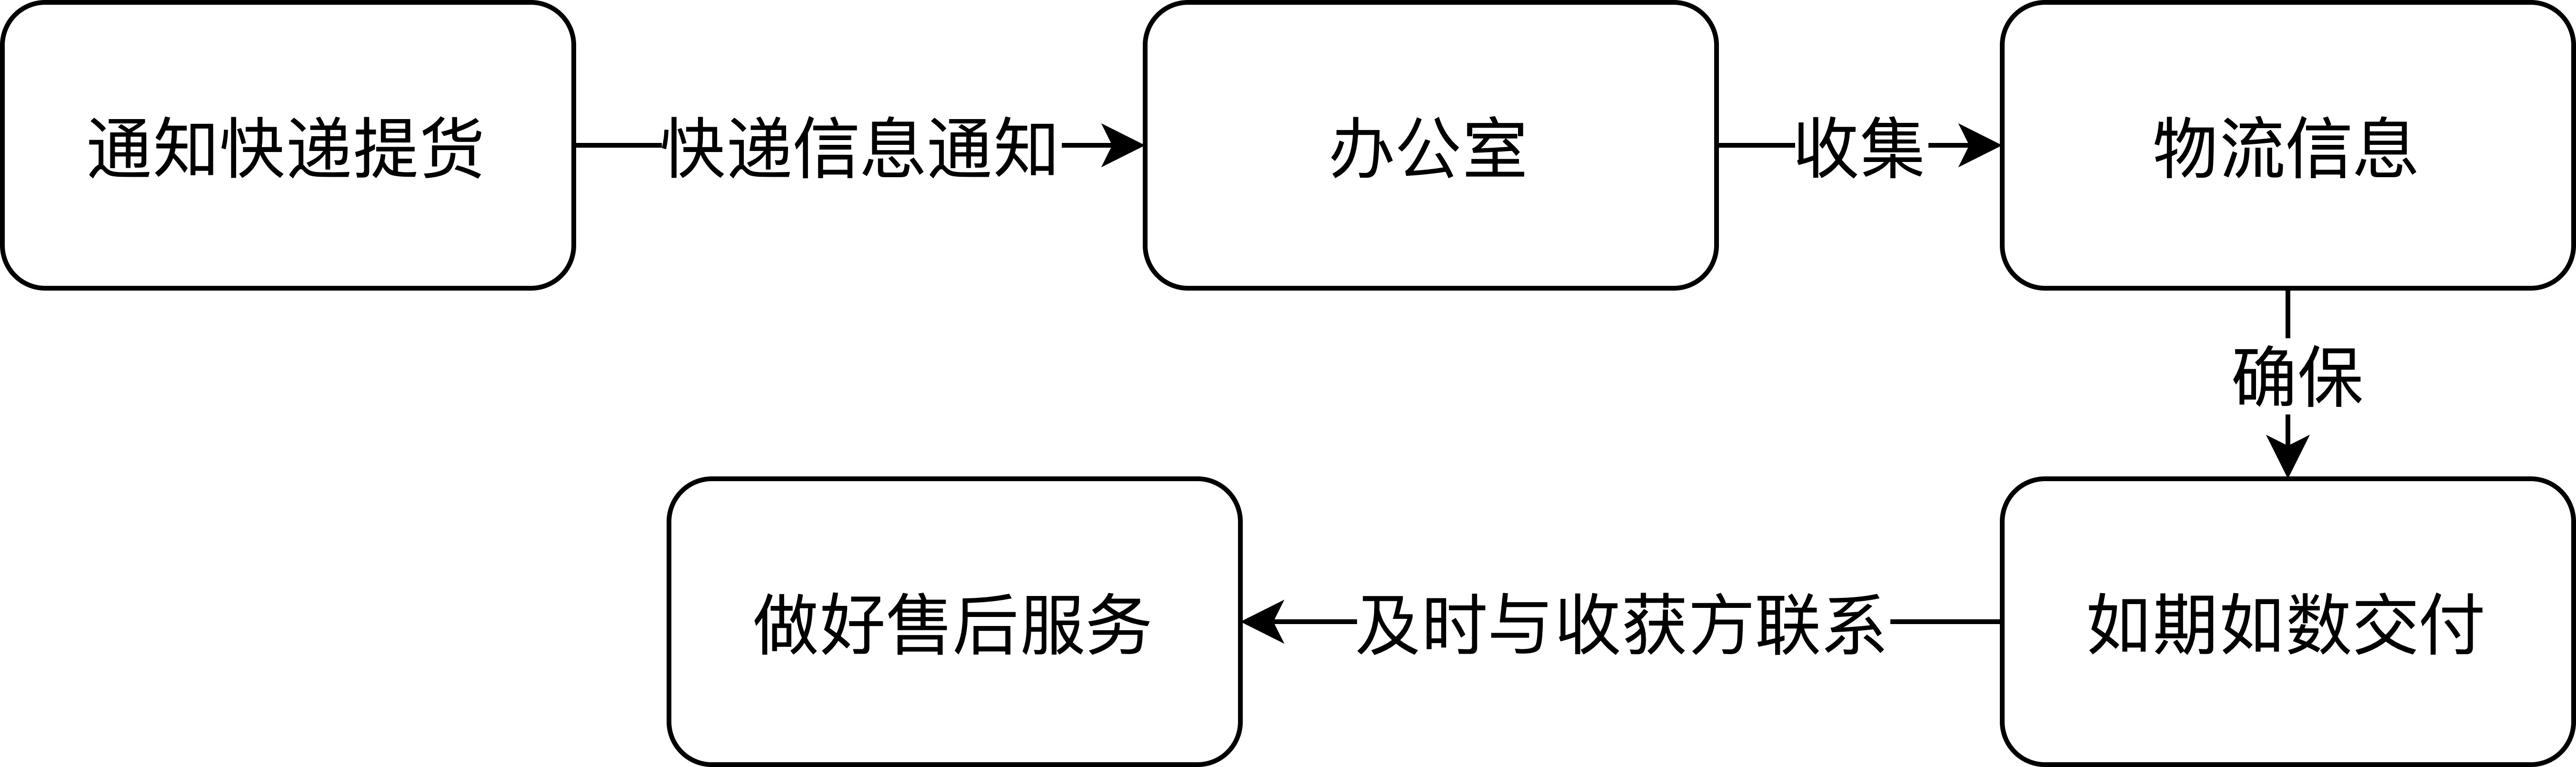
\includegraphics[width=0.7\textwidth]{image/Transport.png}
    \caption{发货要求}
    \label{TR}
\end{figure}

\section{生产准备过程实践}

在开始一批产品的生产前,需要进行生产前的各项准备。本次实习生产前的各项准备是于7月23日上午进行的,主要进行了耗材的补充、仪器及耗材的灭菌、消毒液的配置和清场工作。

\subsection{耗材的补充}
实验中最常用到的耗材为移液器枪头(下面简称枪头),为防止污染和方便枪头的灭菌与使用,在实验室和车间中,枪头一般被有序存放在枪头盒中。

从外界购买的枪头可以是已经有序插入到枪头盒中的成品,但是由于成本原因,一般公司会选择袋装的枪头。因而,在补充耗材期间,需要将购得的散装枪头依次插入枪头盒中。插好的枪头盒需要在开口处贴上灭菌指示胶带,该胶带在高压灭菌锅中处理足够长的时间后,其表面的绿色条纹会变为黑色,从而指示灭菌温度和时间达到要求。

此外,对于实验中常用的EP管,也要将其装入不锈钢盒中,贴上灭菌指示胶带,送入高压灭菌锅中进行使用。

\subsection{仪器及耗材的灭菌}

本次实习进行灭菌的仪器和耗材主要为枪头、EP管以及96孔板。使用的方法为湿热灭菌法,灭菌所用的设备为高压灭菌锅,灭菌后使用烘箱进行烘干。

使用高压灭菌锅前,应按照SOP文件进行仔细的检查,主要检查水位和阀门的情况。当检查无误后,设置灭菌的温度和时间(本次为\SI{121}{\celsius},\SI{20}{\minute}),放入待灭菌的物品,\textbf{打开排气阀}。待灭菌锅升温至\SI{105}{\celsius}后,关闭排气阀。

灭菌完成后,取出灭菌后的物品,放入烘箱中,\SI{65}{\celsius}烘干\SI{6}{\hour}即可。

\subsection{消毒液的配置}

该公司常用的消毒液有两种:75\%酒精消毒液和84消毒液。配置消毒液的过程如下。

\begin{itemize}
    \item 撕去分装瓶上的标签,弃去上一次配置后没有使用完的消毒液。
    \item 按配方配制消毒液。(酒精直接在分装瓶里配置,84消毒液需在容量瓶中定容)
    \item 书写标签,注明消毒液的种类,配置时间和失效时间。一般而言,酒精消毒液的有效期为15天,而84消毒液的有效期为7天。
\end{itemize}

\subsection{场地清洁}

在完成一个批次的产品生产后或者即将进行产品生产前,需要对生产车间和检验实验室进行清场操作,用于预防上一批次的产品对该生产批次的污染。

清场操作主要包括,整理桌面,擦拭桌面、设备、仪器、门窗和墙面,清扫地面,拖地等。其中,擦拭不同部分所用的抹布用不同的颜色区分,如擦拭设备的抹布为红色,而擦拭桌面的抹布为黄色等。


\section{生产过程实践}

\subsection{产品生产}

\subsubsection{万级车间的生产}

\paragraph{万级车间的产品} 主要为阳性对照。由于阳性对照可能污染其他生产区域,进而导致试剂盒成品出现假阳性的情况,故而阳性对照的样品,在相对负压的万级车间进行生产。相关人员应当遵守万级车间的操作规范,穿着连体防护服进入生产区域。

\paragraph{生产流程} 大致为人员及物料准备,清场,溶液混合,溶液分装,灯检,半成品入库,清场。具体如下所示。
\begin{enumerate}
    \item 人员及物料准备:填写相关文件,人员按照车间要求进行穿戴,物料经过传递窗传入车间生产区域。
    \item 清场:打开生物安全柜的紫外灯15分钟,然后依次用84消毒液和酒精消毒液擦拭台面及移液枪。
    \item 溶液混合:计算各溶液的用量,混合于离心管中,稍稍摇晃混匀。
    \item 溶液分装:按生产文件要求,调整电动移液器,然后将溶液分装到半成品管中,盖好管盖。
    \item 灯检:将半成品置于灯检的仪器下,观察液面是否齐平,溶液是否澄清。
    \item 半成品入库:将灯检合格的半成品放入自封口袋中,办理入库。
    \item 清场:整理台面,依次用84消毒液和酒精消毒液擦拭台面及移液枪,打开车间中的紫外灯。
\end{enumerate}

\subsubsection{十万级车间的生产}

基本与万级车间相同,着重为分体防护服。

\paragraph{十万级车间的产品} 主要为反应液,酶混合液以及阴性对照。基于十万级车间的洁净度要求,该车间需要保持高于外界环境\SI{20}{\kilo\pascal}的压力,且相关人员应当遵守十万级车间的操作规范。

\paragraph{生产流程} 大致为人员及物料准备,清场,溶液混合,溶液分装,灯检,半成品入库,清场。具体如下所示。
\begin{enumerate}
    \item 人员及物料准备:填写相关文件,人员按照车间要求进行穿戴,物料经过传递窗传入车间生产区域。
    \item 清场:打开生物安全柜的紫外灯15分钟,然后依次用84消毒液和酒精消毒液擦拭台面及移液枪。
    \item 溶液混合:计算各溶液的用量,混合于离心管中,稍稍摇晃混匀。
    \item 溶液分装:按生产文件要求,调整电动移液器,然后将溶液分装到半成品管中,盖好管盖。
    \item 灯检:将半成品置于灯检的仪器下,观察液面是否齐平,溶液是否澄清。
    \item 半成品入库:将灯检合格的半成品放入自封口袋中,办理入库。
    \item 清场:整理台面,依次用84消毒液和酒精消毒液擦拭台面及移液枪,打开车间中的紫外灯。
\end{enumerate}

\subsection{产品贴签}
成品中,各组成部分装有试剂的可利管(Legris tube)上须贴上标签,标明其对应于说明书中的哪种试剂,并标注批号和失效日期。产品贴标签的流程大致如下。

\begin{enumerate}
    \item 从半成品库取出待贴标签的半成品以及标签纸,插片,并填写相关记录。
    \item 清理桌面,先将插片插入可利管。
    \item 将标签贴在可利管中部,注意不要贴反,贴歪。
    \item 检查贴好标签的半成品。
\end{enumerate}
注意,该过程应当迅速进行,因为在贴标签过程中,产品从冷库转移到室温下进行操作,因而酶等组分容易失活。笔者的同学进行贴标签时的工作状态如下图所示。

\begin{figure}[H]
    \centering
    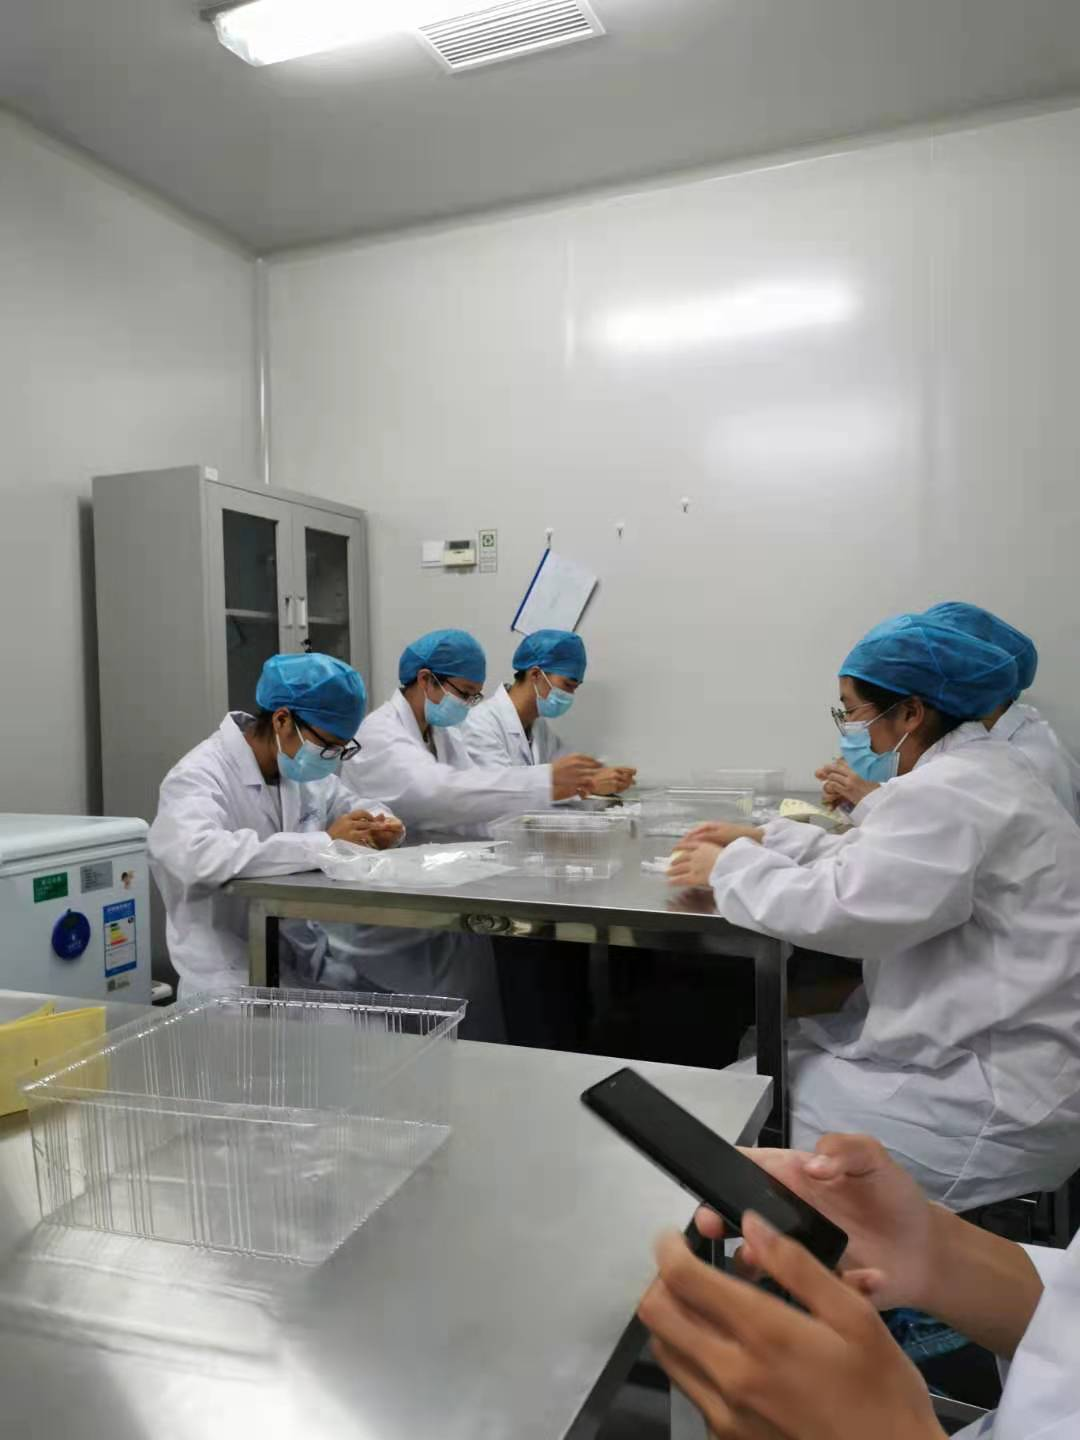
\includegraphics[width=0.5\textwidth]{image/WechatIMG25.jpeg}
    \caption{贴标签时的同学们}
    \label{STAFF}
\end{figure}

\subsection{产品组装}

贴好标签的可利管依次放入包装盒的内衬中,加入说明书,封口后组成成品。

整个流程较为复杂,因而使用流水线作业的方式比较合理且高效,流水线的组成分为几块:
\begin{enumerate}
    \item 折叠说明书
    \item 准备并安装衬里
    \item 按要求放置各类试剂管
    \item 放置说明书
    \item 检查组装的成品
    \item 进行封口
\end{enumerate}

\begin{figure}[H]
    \centering
    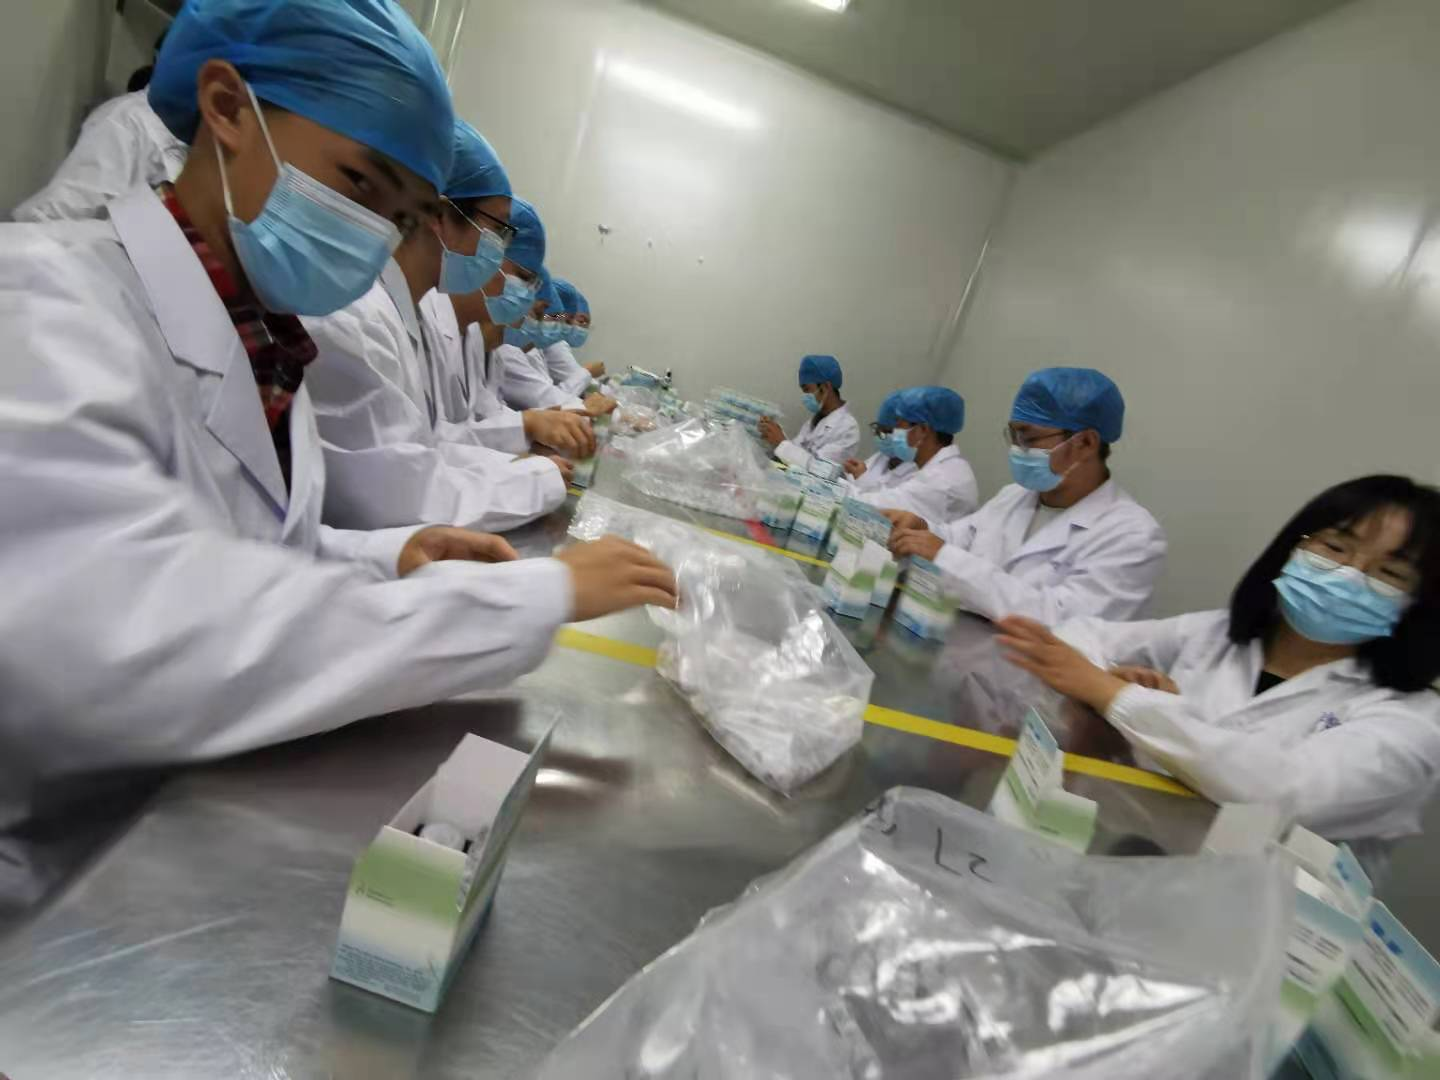
\includegraphics[width=0.7\textwidth]{image/WechatIMG26.jpeg}
    \caption{组装产品时的同学们}
    \label{STAFF}
\end{figure}


\section{检验过程实践}

\subsection{产品原料检验(直接检)}

\subsubsection{检验原理}
考虑到产品原料历来的合格率,结合对于检验的设备的成本以及检验简便性的需求,对于本次生产的产品的原料检验,一般不采取分光光度法、凝胶电泳和测序等复杂的方法,而是直接配置成10人份的小样,与标准试剂混合后进行rtPCR(相当于制作了一批产品并进行全数检验)。若rtPCR给出的结果符合预期,则可以认为原料质量满足生产需求。

关于rtPCR的原理,相见上文本次生产产品介绍部分的内容。

\subsubsection{PCR实验室布局}

\begin{figure}[H]
    \centering
    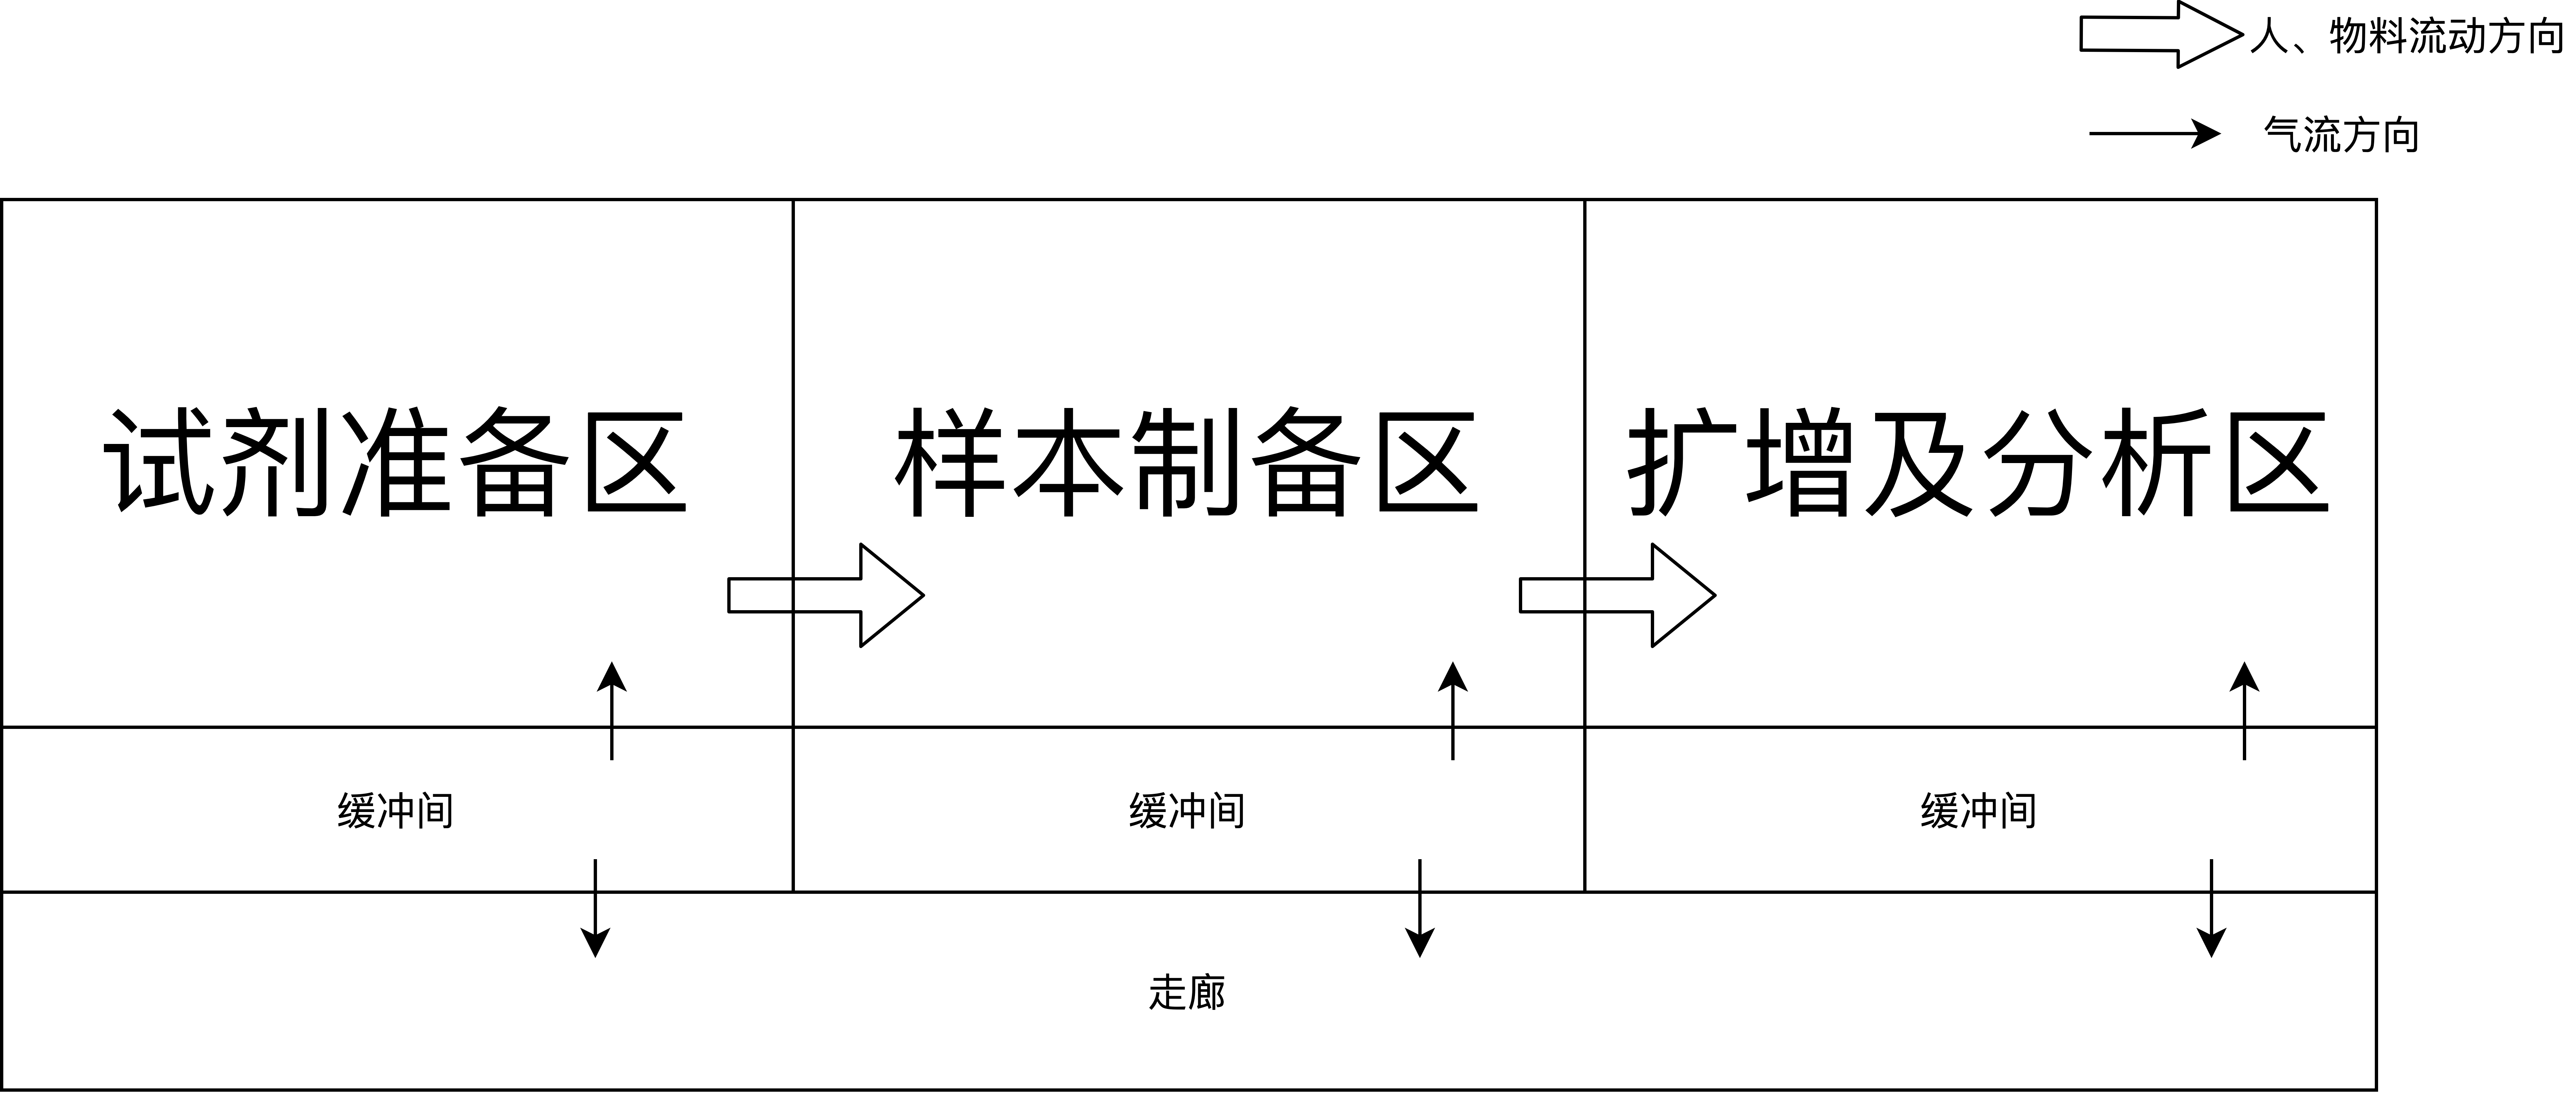
\includegraphics[width=0.7\textwidth]{image/PCR_Lab_Layout.png}
    \caption{PCR实验室布局}
    \label{PCR}
\end{figure}

\subsubsection{检验过程}

检验的过程主要分为三个部分,与PCR实验室的布局相对应。

\paragraph{反应体系的配置} 在试剂准备区混合dNTP,引物,探针,Taq酶,UNG酶,以及对应的缓冲溶液;共配置7组不同的反应体系,每组反应体系加入\SI{18}{\micro\liter}到八连排管中。

\paragraph{标准样品的准备与上样} 在样品制备区向\SI{10}{\micro\liter}阳性样品中加入\SI{10}{\micro\liter}缓冲液和\SI{80}{\micro\liter}纯水,混匀后加入\SI{500}{\micro\liter}DNA提取液,\SI{100}{\celsius}处理5分钟,12000转离心1分钟,即得阳性对照。取\SI{10}{\micro\liter}低浓度的标准样(EP管标号为S*2的管),加入\SI{90}{\micro\liter}纯水稀释,混匀后离心3秒,即得用于测验检出限的标准样。每组八连管中,按照高浓度标准样,低浓度标准样,检出限标准样,检出限标准样,阳性对照,阴性对照,阴性对照,阴性对照的顺序,向每小管反应体系中加入\SI{2}{\micro\liter}样品。

\paragraph{rtPCR仪器的设置} 按SOP文件设置rtPCR仪的运行参数,本次使用的是ABI 7000 Real Time PCR仪,设置好四个通道数,样品性质(待测,阴性,阳性),样品所在区域,升降温程序,荧光采集位置等项目后,运行扩增。

\subsubsection{检验结果}

根据rtPCR仪器给出的结果,参照该公司的文件,可以判断原料基本合规,可以用于下面的生产。具体表现为:

\begin{enumerate}
    \item 所有荧光信号较强的曲线均为标准的rtPCR中的sigma型曲线,而没有信号的曲线几乎为平行的直线。
    \item 各标准品组的Ct值满足要求。
    \item 检出限标准品的曲线几乎重合,说明该原料生产的试剂重复性好。
    \item 阳性对照组的曲线和检出限标准品相差较少,说明样本处理和提取过程中没有出现问题。
    \item 阴性对照组大部分满足要求,仅有个别组在38轮扩增后出现少许荧光信号,推测为非特异性扩增,或实验室环境中气溶胶的污染。
\end{enumerate}
对于阴性对照组大中个别组在38轮扩增后出现少许荧光信号的问题,由于问题不普遍,且难以准确确定问题发生的原因,因而可以认为是检测中的偶然误差。可以认为原料质量合格,可以投入生产。

\begin{figure}[H]
    \centering
    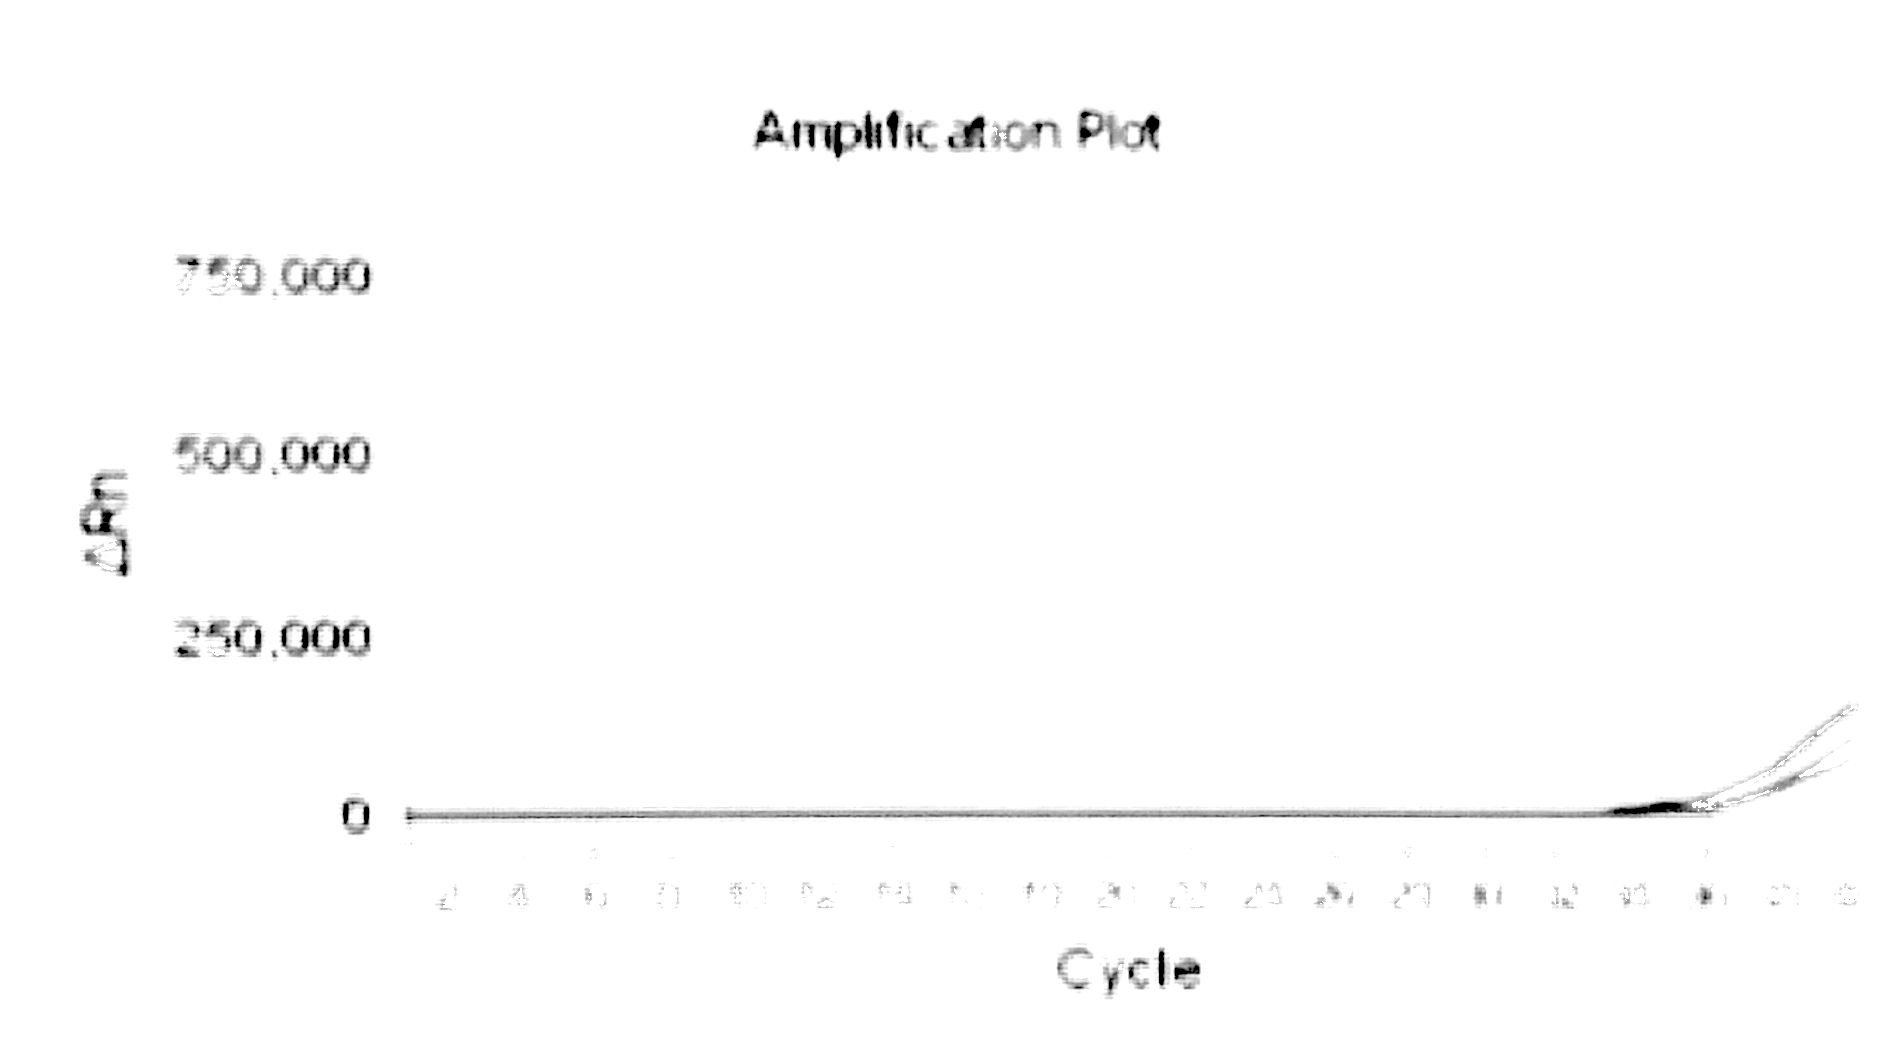
\includegraphics[width=0.6\textwidth]{image/WechatIMG23.jpeg}
    \caption{rtPCR中扩增曲线翘尾的一个例子}
    \label{rtres}
\end{figure}

\subsubsection{检验操作过程中的注意事项}

该检验实验看似相当于学校实验室中较为简单的rtPCR实验,但是考虑到工业生产的诸多要求,其注意事项远远要比学校实验室严格。具体的一些注意举例事项如下。
\begin{itemize}
    \item 操作者应符合洁净环境的着装规范。
    \item 进行一批操作前,以及完成操作后需要用84消毒液和酒精清洁移液器及台面。
    \item 使用Vortex混匀液体,然后需进行3秒左右的离心。
    \item 溶液配置与加入的顺序需按照SOP文件的指导进行。
    \item 优先打出枪头中的液体,其次是关闭EP管盖。
    \item 八连管盖在操作完成前,只要按紧收尾两个即可,可以防止中间操作的液体沾到管盖上造成污染。
    \item 移液枪操作时,尽量按照规定的路线进行,避免污染。
\end{itemize}

\subsection{纯化水检测}

\subsubsection{检验原理}
参考上文以及《中国药典》2020版通则1105,以及\texttt{YY/T 1244-2014} 《体外诊断试剂用水》。

\subsubsection{检验过程}
\paragraph{纯化水检验项目} 主要包括:性状,酸碱度,易氧化物,电导率,微生物限度。检验项目的具体要求及细节如下所示。
\begin{enumerate}
    \item 形状:无色澄清液体;无臭,无味。
    \item 酸碱度:使用甲基红和溴麝香草酚蓝进行定性检测。\SI{10}{\milli\liter}纯化水中加入2滴甲基红指示剂,体系不得为红色。\SI{10}{\milli\liter}纯化水中加入5滴溴麝香草酚蓝指示剂,体系不得为蓝色。检测使用的指示剂为采购的标准品。
    \item 易氧化物:使用高锰酸钾滴定液进行定性检测。按购买的滴定液说明书,纯化水酸化后加入滴定液,煮沸一定的时间后粉红色不得完全消失。
    \item 电导率:使用带有温度补偿功能的电导率测定仪进行测定,按药典标准。
    \item 微生物限度:滤膜法处理后,使用R2A琼脂培养基,于\SI{30}{\celsius}至\SI{35}{\celsius}培养不少于5天,依据药典检查,细菌总数不应超过50CFU/mL。
\end{enumerate}

\subsubsection{检验操作过程中的注意事项}
取水时,若要进行微生物限度检验,则应当取\SI{900}{\milli\liter}于容器中,容器做好标识;若要进行其他检验,则\SI{300}{\milli\liter}为合适的取水量。

\subsection{万级环境检测}

\subsubsection{检验原理}
参考上文以及相关法律法规。法规依据主要如下。
\begin{itemize}
    \item GB 50073-2013 洁净厂房设计规范
    \item GB/T 16292-2010 医药工业洁净室(区)悬浮粒子的测试方法
    \item GB/T 16293-2010 医药工业洁净室(区)浮游菌的测试方法
    \item GB/T 16294-2010 医药工业洁净室(区)沉降菌的测试方法
\end{itemize}

\subsubsection{检验过程}
\paragraph{洁净环境检验项目} 主要包括:尘埃粒子数,微生物限度,换气次数,相对湿度,静压差,温度与照明度。其中,尘埃粒子数,微生物限度和换气次数的检验为平均每月一次;相对湿度,静压差和温度为每班一次;而由于灯光条件较为稳定,照明度的检测为每季度一次。各项目的检测标准大致如下。

\begin{enumerate}
    \item 尘埃粒子数:采样点力求均匀,采样高度略高于工作面。按洁净度级别不同,标准不同,具体数值参照相关法规。
    \item 微生物限度:包括浮游菌和沉降菌。沉降菌与尘埃粒子数的采样方式类似,浮游菌需通过抽气过滤处理进行采样,按洁净度级别不同,标准不同,具体数值参照相关法规。
    \item 相对湿度,静压差和温度:读取待测区域的相关仪器,做好记录。
    \item 照明度:使用电子照度计进行测量,公司要求为不低于 150 lux。
    \item 换气次数:测量风机的进风速度,除以空间的容积即可。
\end{enumerate}

\subsubsection{检验操作过程中的注意事项}
进行尘埃粒子数检测时,保证检测环境中尽可能存在少的人员,应当设置好仪器的时间,将取样量调整为经验值\SI{2.85}{\liter};按下检测按键后,人员随即离开待检测的环境,关上门后等待结果被打印出。

进行换气次数检测时,应当让身高合适的人员进行。使用风量仪时,应当确保待测出风口被完全罩入风量仪中,避免测量误差。

\subsection{产品成品检验}

本次检验的两种成品,一种为27分型的产品,为本次实习所生产;另一种为15分型产品,为仓库留样,已经过期两年多。留样产品的检验主要意在测试其极限情况下的稳定性,及其有效期外的

\subsubsection{检验原理}
主要为rtPCR,与原料检几乎完全相同,这里不再赘述了。

\subsubsection{检验过程}
分为反应体系配置,样本处理以及扩增分析三大块,与原料检几乎完全相同,这里不再赘述了。

\subsubsection{检验结果}
根据rtPCR仪器给出的结果,参照该公司的文件,可以判断本批次产品(27分型)合格。

对于15分型的试剂,由于该试剂已经存放三年,过期时间较长,部分分型(例如HPV-56)的探针荧光性能不佳(Ct值不合格)。

具体表现为:
\begin{enumerate}
    \item 所有荧光信号较强的曲线均为标准的rtPCR中的sigma型曲线,而没有信号的曲线几乎为平行的直线。
    \item 各标准品组的Ct值满足要求。
    \item 检出限标准品的曲线几乎重合,说明该原料生产的试剂重复性好。
    \item 阳性对照组的曲线和检出限标准品相差较少,说明样本处理和提取过程中没有出现问题。
    \item 阴性对照组大部分满足要求,但在15分型的检验时,出现了普遍的CY5通道低水平的扩增,出现原因可能与样品制备时的交叉污染有关,但具体原因还需额外设计实验。
\end{enumerate}

下图展示了不同检测浓度下的曲线,如图所示,各种检测浓度和检测限的曲线区别较为明显。
\begin{figure}[H]
    \centering
    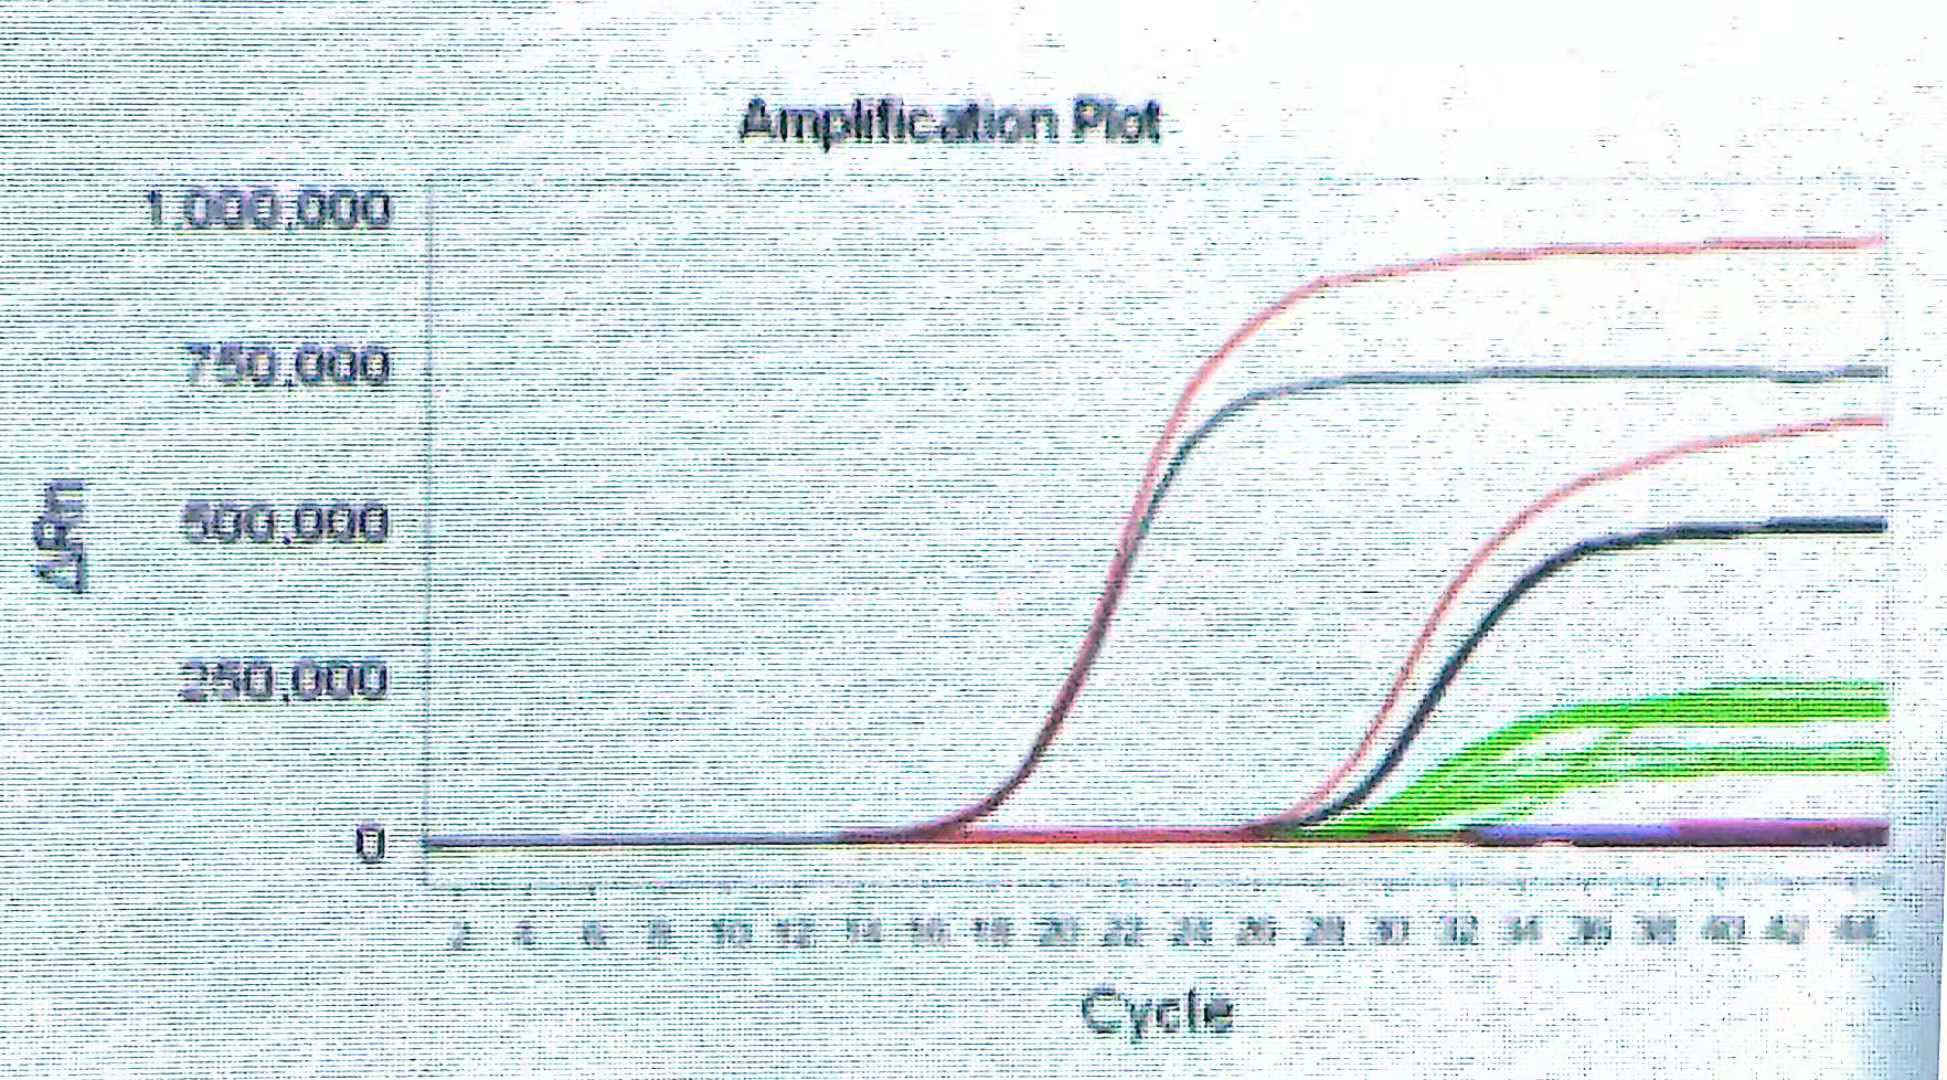
\includegraphics[width=0.6\textwidth]{image/WechatIMG28.jpeg}
    \caption{rtPCR中不同浓度的质控品在同一反应体系中扩增曲线的一个例子}
    \label{rtres}
\end{figure}

下图展示了某个精密度检验的结果,可见,10条扩增曲线几乎重合,精密度较好。
\begin{figure}[H]
    \centering
    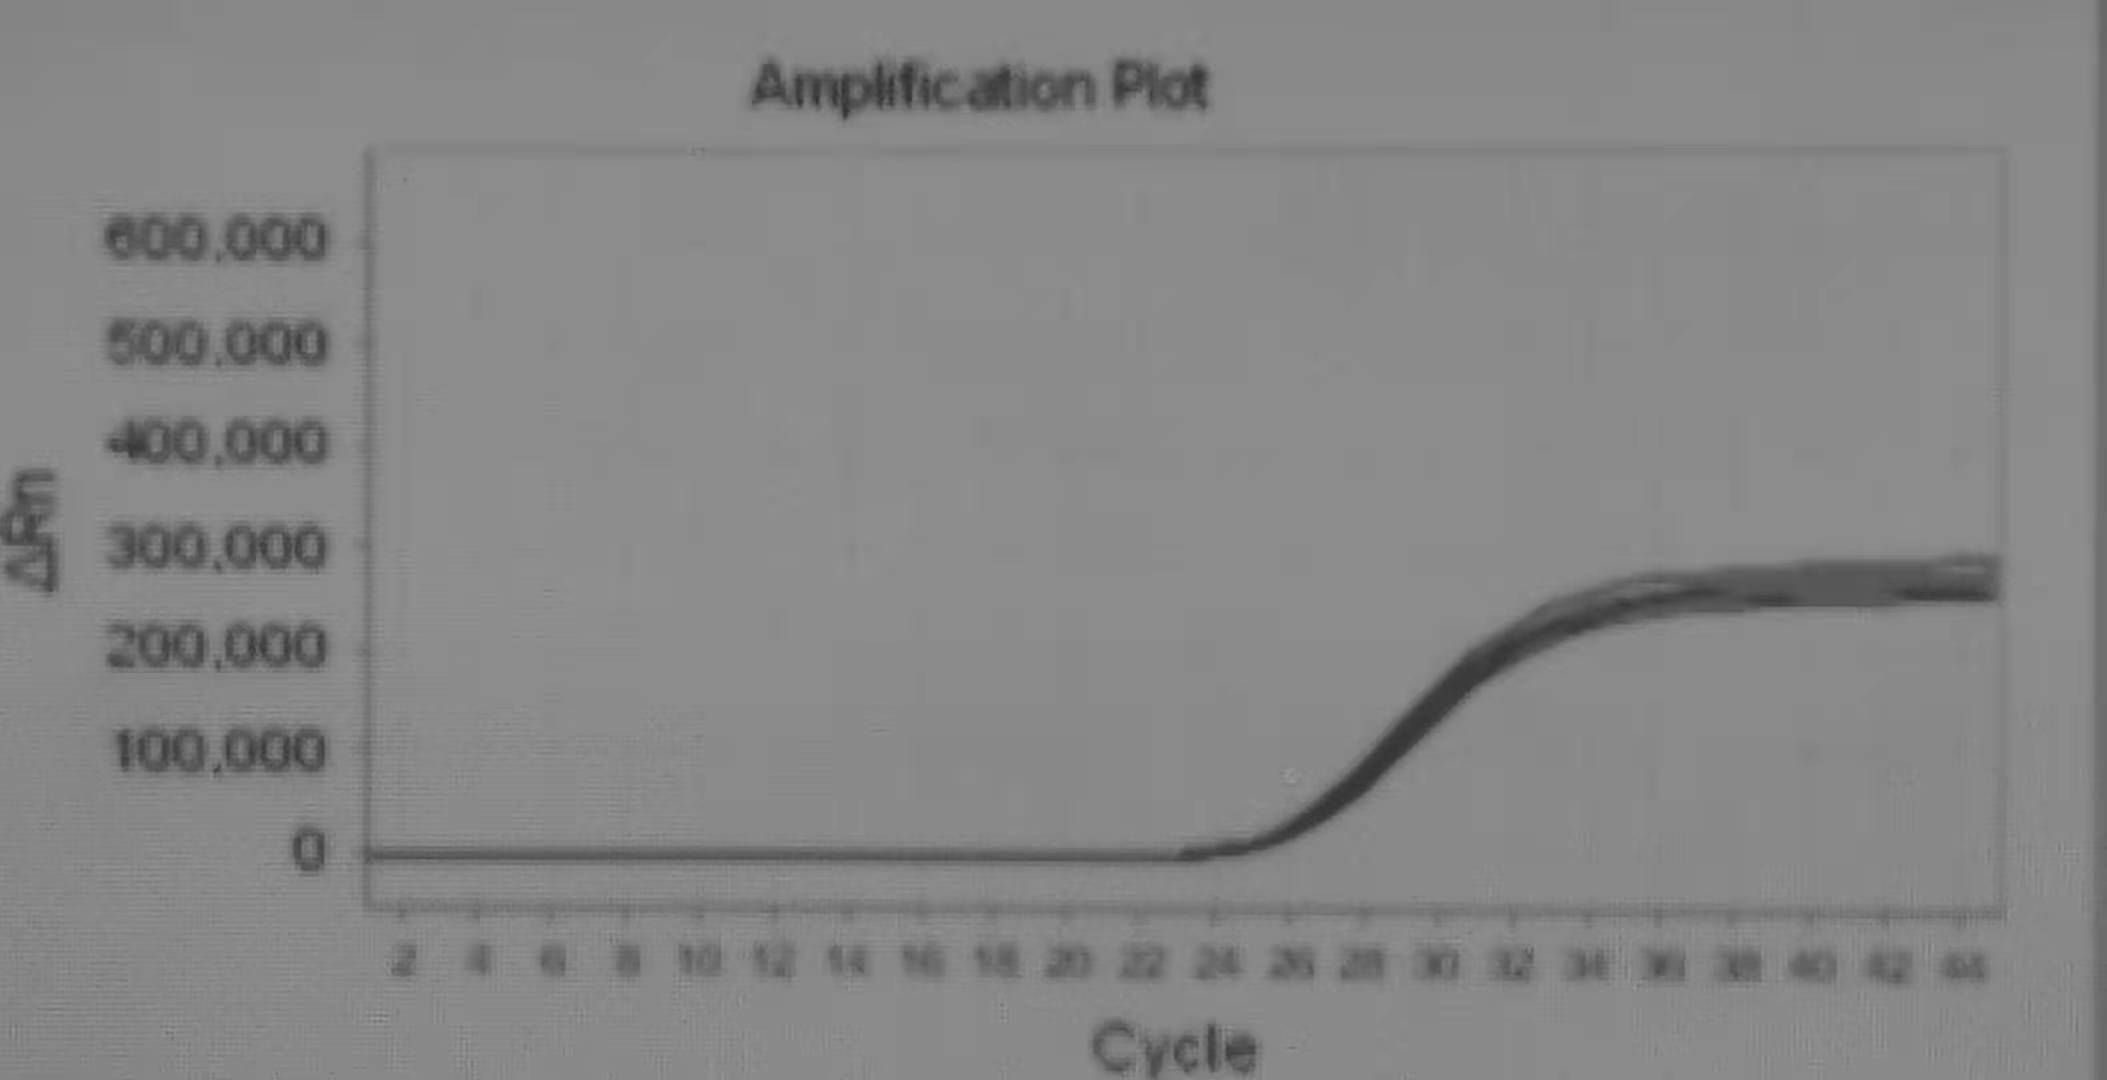
\includegraphics[width=0.6\textwidth]{image/WechatIMG29.jpeg}
    \caption{精密度检验中的一组扩增曲线}
    \label{rtres}
\end{figure}





\section{对于实习所在公司的交流与思考}

实习过程中,笔者注意到所在公司与笔者曾经所参观过的高校、研究所、企业的管理与实际实验操作中有一些不同。笔者针对这些不同点向带教的公司员工进行了一些交流,一部分内容摘录于下。

\paragraph{关于PCR实验室的分区} 该公司的PCR实验室分为三个房间,分别用于配制反应液,处理待测样本以及进行扩增与分析。其中,人员和物料的移动只能从底核酸污染区域向高核酸污染区域进行,且物料的传递需要使用传递窗进行。反应液配置与样品提取则需要分别在超净工作台和生物安全柜中进行。

相比于笔者在校内的PCR实验室,该公司的实验室明显复杂许多,而且管理极为严格。笔者在校内进行rtPCR实验,反应体系的配置、样品处理与PCR仪在同一房间,且反应体系的配置与样品处理在同一实验台进行,PCR仪则放置于另一试验台,中间几乎没有严格的隔离与污染防治措施。正常进行PCR实验时,笔者在学校中会被要求戴口罩,并不时向手及周围空间喷洒消毒液以防止污染。

与该公司员工交流后得知,rtPCR作为一种极其敏感的检测方法,检出限可以达到几个核算分子级别,故而除了需要防止液体造成的污染外,气溶胶污染也需要防治,因而将PCR实验室分为不同区域,且设置不同的换气排气方式,以避免污染。此外,rtPCR作为公司的重要指控手段,其准确性必须得到保证,因而进行严格的污染防控是及其必要的。相比之下,学院和科研院所的rtPCR主要用于探索并表征某些未知基因的表达量,而非用于涉及到安全问题的工业生产中,对于检出限和准确性要求不高,因而为降低科研成本,方便操作,提高实验效率,故而防治污染的手段就较为粗糙一些。

\paragraph{关于实验室的设备布局} 在进行各类检测实验时,笔者注意到,相比于笔者所在课题组的实验室,该公司实验室的设备摆放的间隔相对较大,空间利用率不高,相同面积实验室功能较为单一。例如,在PCR实验室的样品处理间内,设置有一个实验台,一个生物安全柜,一个超净工作台。其中,实验台上放有Vortex一台,离心机一台,EP管架一板,吸水纸一包;生物安全柜和超净工作台中放有消毒剂喷雾,干式加热器一台,枪头盒一到二盒,移液枪架一个,以及配套的5把不同规格的移液枪。整体环境较为空旷,相同大小的空间若放在笔者的实验室,则至少可以放入一整套分子操作的设备(电泳槽,PCR仪,凝胶成像仪,各类耗材等)。

与公司员工交流后发现,实验室中设备等布局除了有相关法律法规等要求外,主要还是考虑到实验室对污染防控的要求较高,因而不得不牺牲部分功能,从而有利于人员在操作时减少失误。此外,较为简单而空旷的实验环境有利于环境的清洁卫生,有利于实验中失误的处理与补救,也能使得工作人员有较为舒适的工作环境。

\paragraph{关于实验室的操作细节} 在进行实验操作的过程中,笔者和笔者的同学时常被公司带教人员提醒,要注意实验操作的细节。其中,很多操作方式在笔者的课题组实验室几乎没有提及。例如,在使用移液枪向八连排管加样时,笔者在课题组的通常做法是,将枪头插入八连管中已有的液体内,多次吹打混匀。而在该公司中,其推荐的方式为,将枪头倾斜插入管中,抵住管壁,一次性打入液体后不松手,保持倾斜角度将枪头移出管子后,再松手,然后打掉枪头,进行下一轮操作。待一组八连管加完后,盖好盖子,放入离心机中离心,使得壁上的液体被甩入下层。此外,在加样时,八连管架一般置于操作者正前方,防止样品的EP管架位于左手边,枪头盒位于EP管架远离操作者的一侧,而废弃的枪头盒则位于右手侧。操作时,移液枪依次进入枪头盒,样品管,八连管,垃圾箱,如下图所示。据该公司员工称,一方面,这样的操作可以避免因操作失误造成的污染,另一方面,相对稳定的工具摆放方式也有利于增加操作的效率。

\begin{figure}[H]
    \centering
    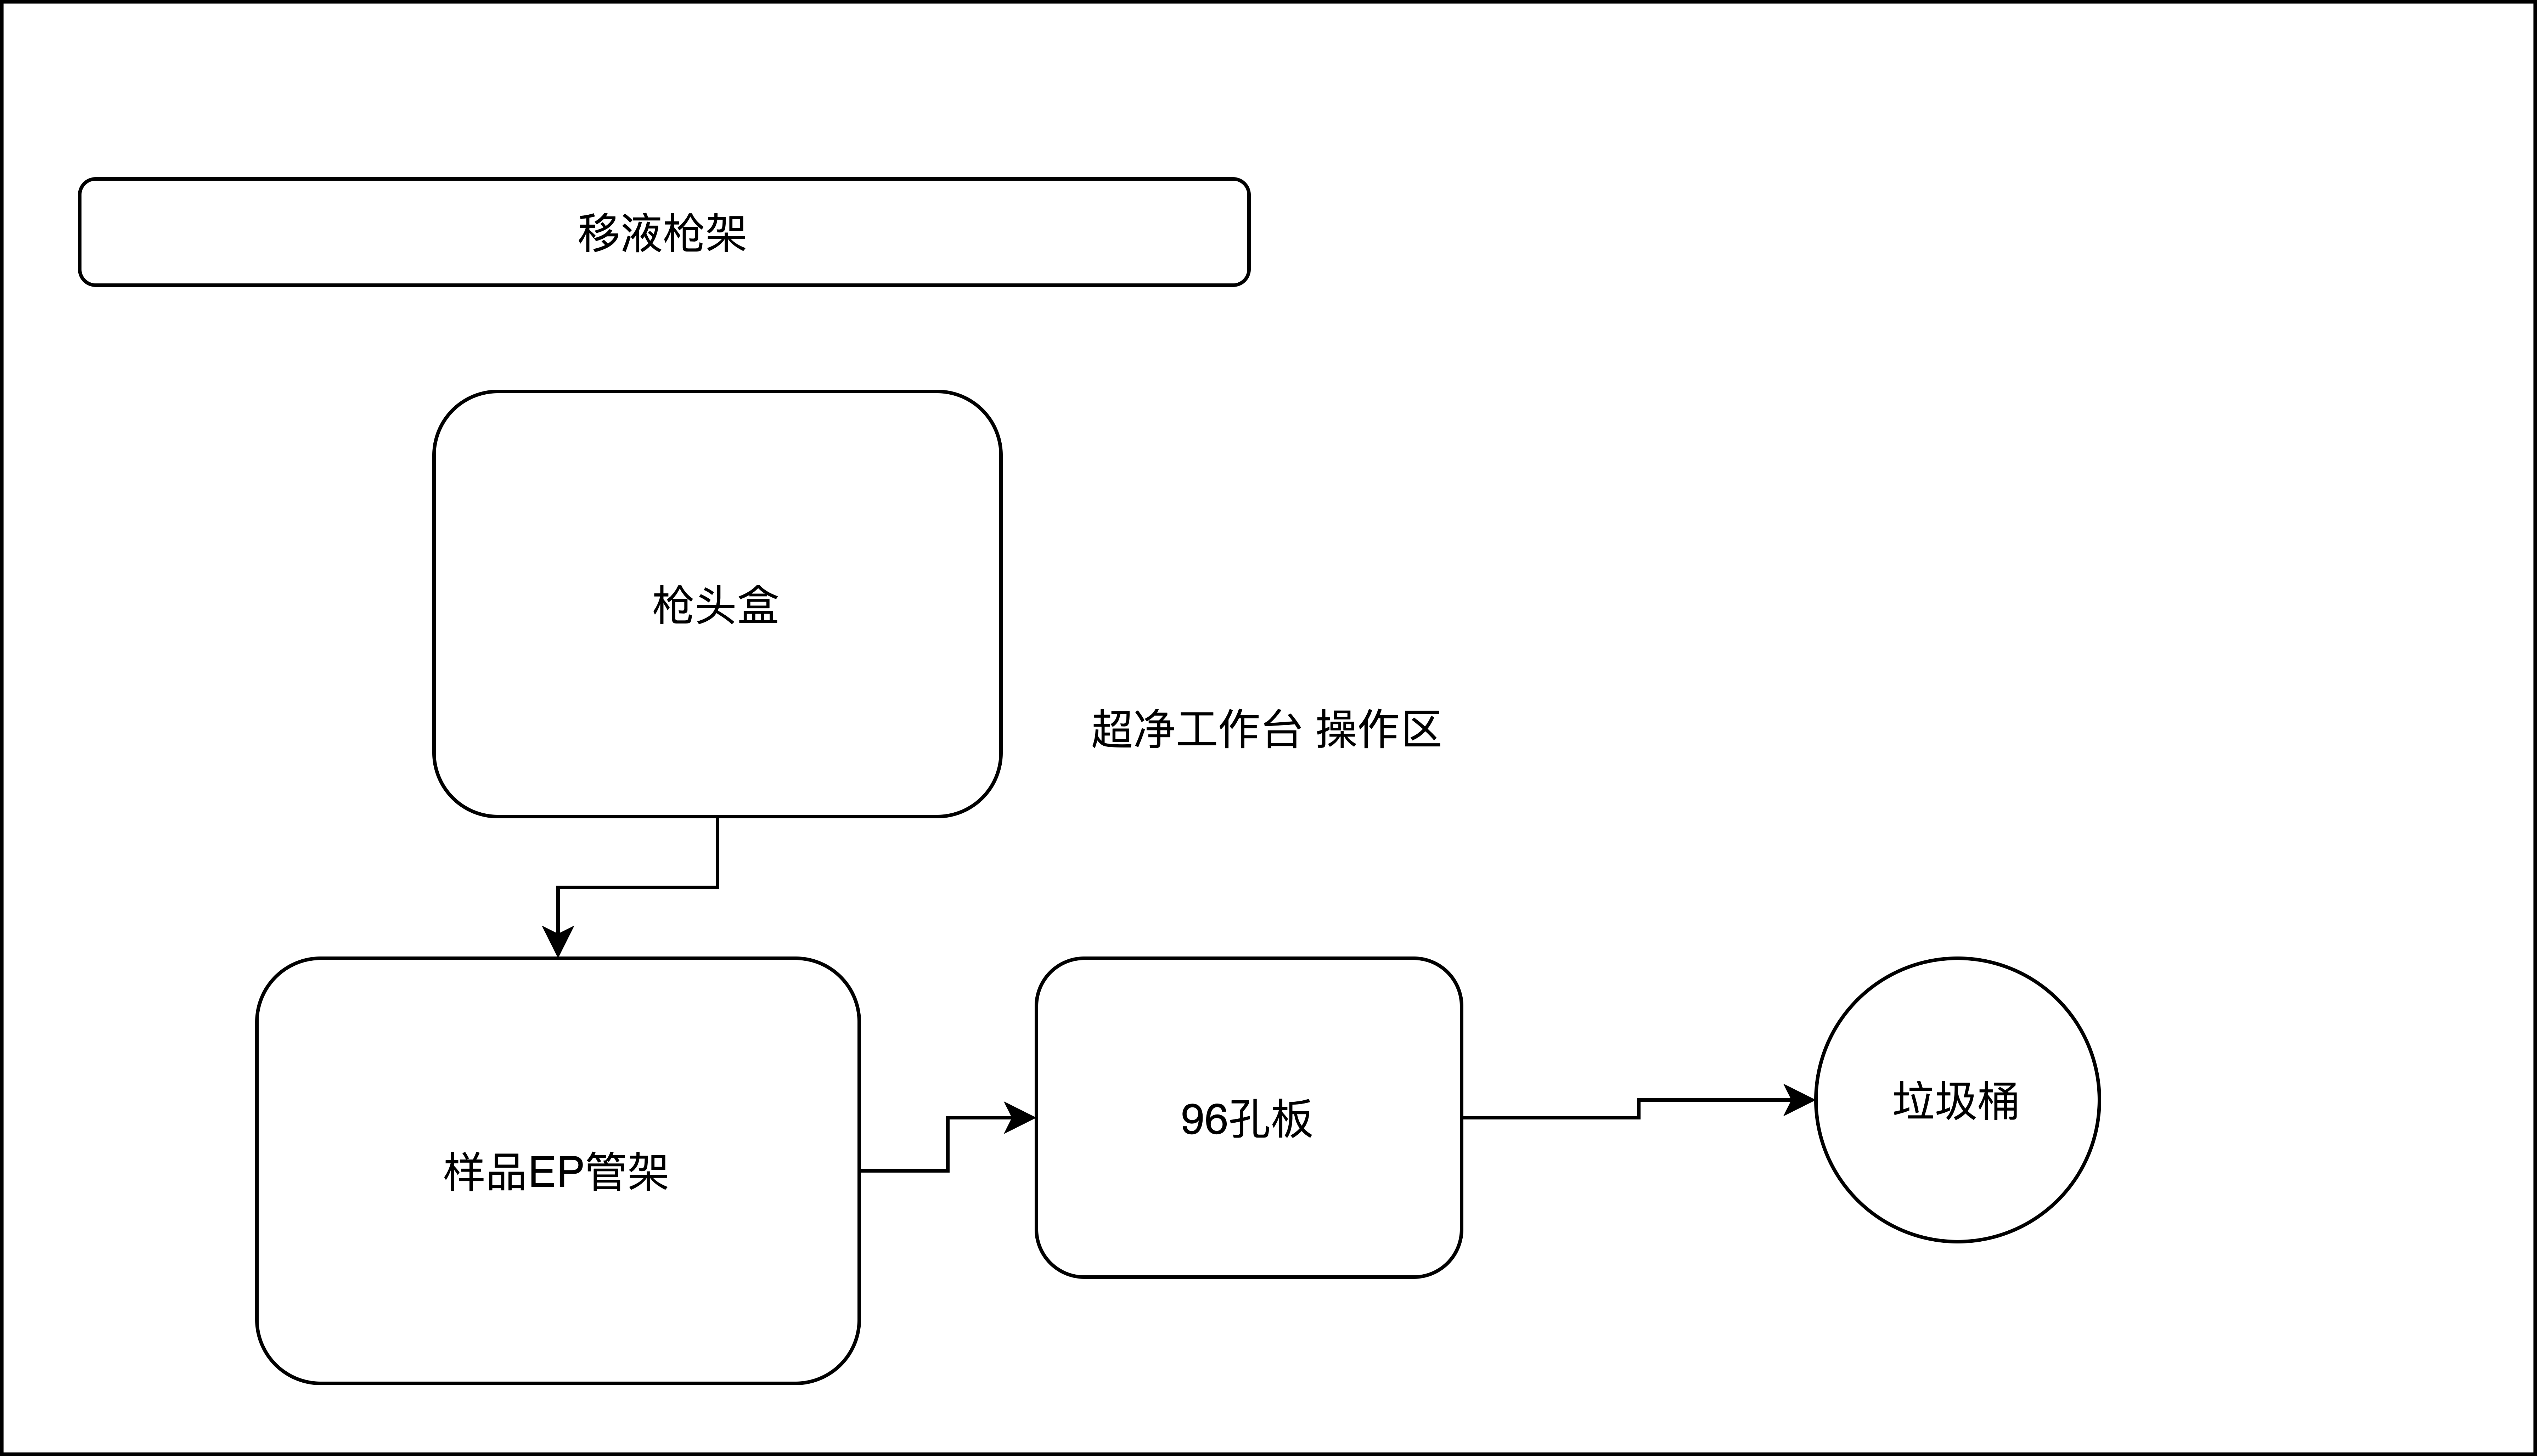
\includegraphics[width=0.7\textwidth]{image/AddMaterial.png}
    \caption{加样时超净工作台中物品的摆放与操作顺序}
    \label{AM}
\end{figure}

\paragraph{}

\paragraph{关于公司实验室的门禁、监控与数字化程度} 笔者在参观该公司的各类设施时注意到,该公司除了进出入车间人员需要进行指纹验证外,其余设施几乎微设置门禁。此外,在公司的实验室、车间与仓库内,均没有发现安装有闭路电视监控。笔者针对门禁和监控到问题与该公司的员工进行交流,得知,该公司由于在职人员较少,规模不大,且作为主要业务为生产销售的公司,对于门禁要求无需过于严格。此外,由于洁净环境里安装监控设备暂时没有明确的规定,因而为了避免上级机构进行检查时到麻烦,故而洁净车间内等均没有安装监控设备。

此外,笔者观察到,该公司的数字化程度不高,且很多设备均没有自动化管理(例如温湿度监测等IoT技术),交流后得知,其主要原因还是成本的考虑。

\paragraph{关于文件管理的方式} 笔者在参加该公司的文件管理培训后,注意到该公司的文件管理,除了与仓库账目相关的部分进行了部分的现代化改造(接入EIP系统等),其余大部分均保持传统的纸质文件管理方式。此外,一些记录性质的文件,仍然保持手动填写的方式。考虑到公司文件数量不大,人员也不多,故而该运作模式较为合理。

与公司员工交流后得知,除了没有必要进行无纸化办公外,公司文件管理需要遵循相关的法律法规,为了应对上级部门的检查,必须采用规定的文件管理方式。此外,传统的纸笔填写、加盖印章、唯一编号的受控文件等方式,有利于维护公司文件的保密与安全,防止文件等真实性出现问题,有利于公司文件记录等可追溯性。

\paragraph{关于SOP文件的编制} 与公司员工进行讨论得知,原则上,SOP文件等应当越细致越好,而且应当步骤明确;然而,若是SOP文件编写过于细致,精确到每一步的操作,虽然方便人员操作,但是对于应对上级机构检查时,如果员工没有严格SOP文件的操作,则会造成不必要的麻烦。此外,人员的操作习惯各有差异,过于细致的SOP文件会对员工造成束缚,从而降低工作效率,而且会扼杀员工的创造力,不利于企业的长期发展。

\paragraph{关于公司产品的推广与销售} 与公司员工进行讨论得知,该公司产品的推广与销售主要分两大块:线下和线上。线下主要依靠市场部进行产品营销的调研(联系医疗检测机构等),推广,营销;线上主要包括通过各类平台(公众号,阿里等)进行推销。值得注意到是,体外检测试剂并不能直接销售给个人用户,一方面,这个特性使得该公司的用户较为单一;另一方面,这个特性也使得推销等过程较为简单。

\paragraph{关于该公司的员工待遇及福利} 与该公司员工交流后得知,该公司员工的平均收入为5k RMB每月,当地房价为平均7k RMB一平米,收入情况不容乐观。工作条件上,除去加班等特殊情况,一般为一周工作40小时,工况尚可,噪音污染不大,但经常会接触有毒有害物质。此外,公司虽然小,但也给员工配备了健身房,台球桌等设施,供员工使用。此外,该公司员工驻留程度高,大多为老员工,但是员工上升空间不是很大。



\section{实习总结与讨论}

本次实习课程中,笔者最大的收获是能够切身体会到学术界与工业界的巨大差距,以及生物相关的产品(如体外诊断试剂盒)从实验室里的论文转化为医疗实践中广泛使用的工具等过程的难度。相比较于学术界,工业界更注重安全性,更注重产品的质量与可靠性,更注重法律法规与管理规范;而这些与生产实践联系紧密的东西,对于处在象牙塔中的本科生来说,是极少能够接触到的。

本次实习中,笔者与同学的交流过程中,得知很多同学对于繁琐的工业界的规范颇有微词,认为其存在会束缚企业的创新能力。而与公司员工的交流的过程中,虽然部分员工对于上级部门的检查也不甚满意,但对于企业的种种规范,他们的评价还是非常正面的:这些规范不是凭空而来,而是基于前人的众多牺牲而总结的经验。

\textit{此外,与公司员工的交流的过程中,不乏有该行业员工待遇普遍不高(远低于互联网等行业)的说法,而且参考他们的薪资标准,工作条件,员工福利与企业规模,也确乎如此。早日得知这种状况,对笔者等本科生以后的职业规划也有重要意义。}

希望学校能够保持公司实习的好传统,从而能切实提高同学们的见识与能力,补齐同学们的知识盲区。

\begin{figure}[H]
    \centering
    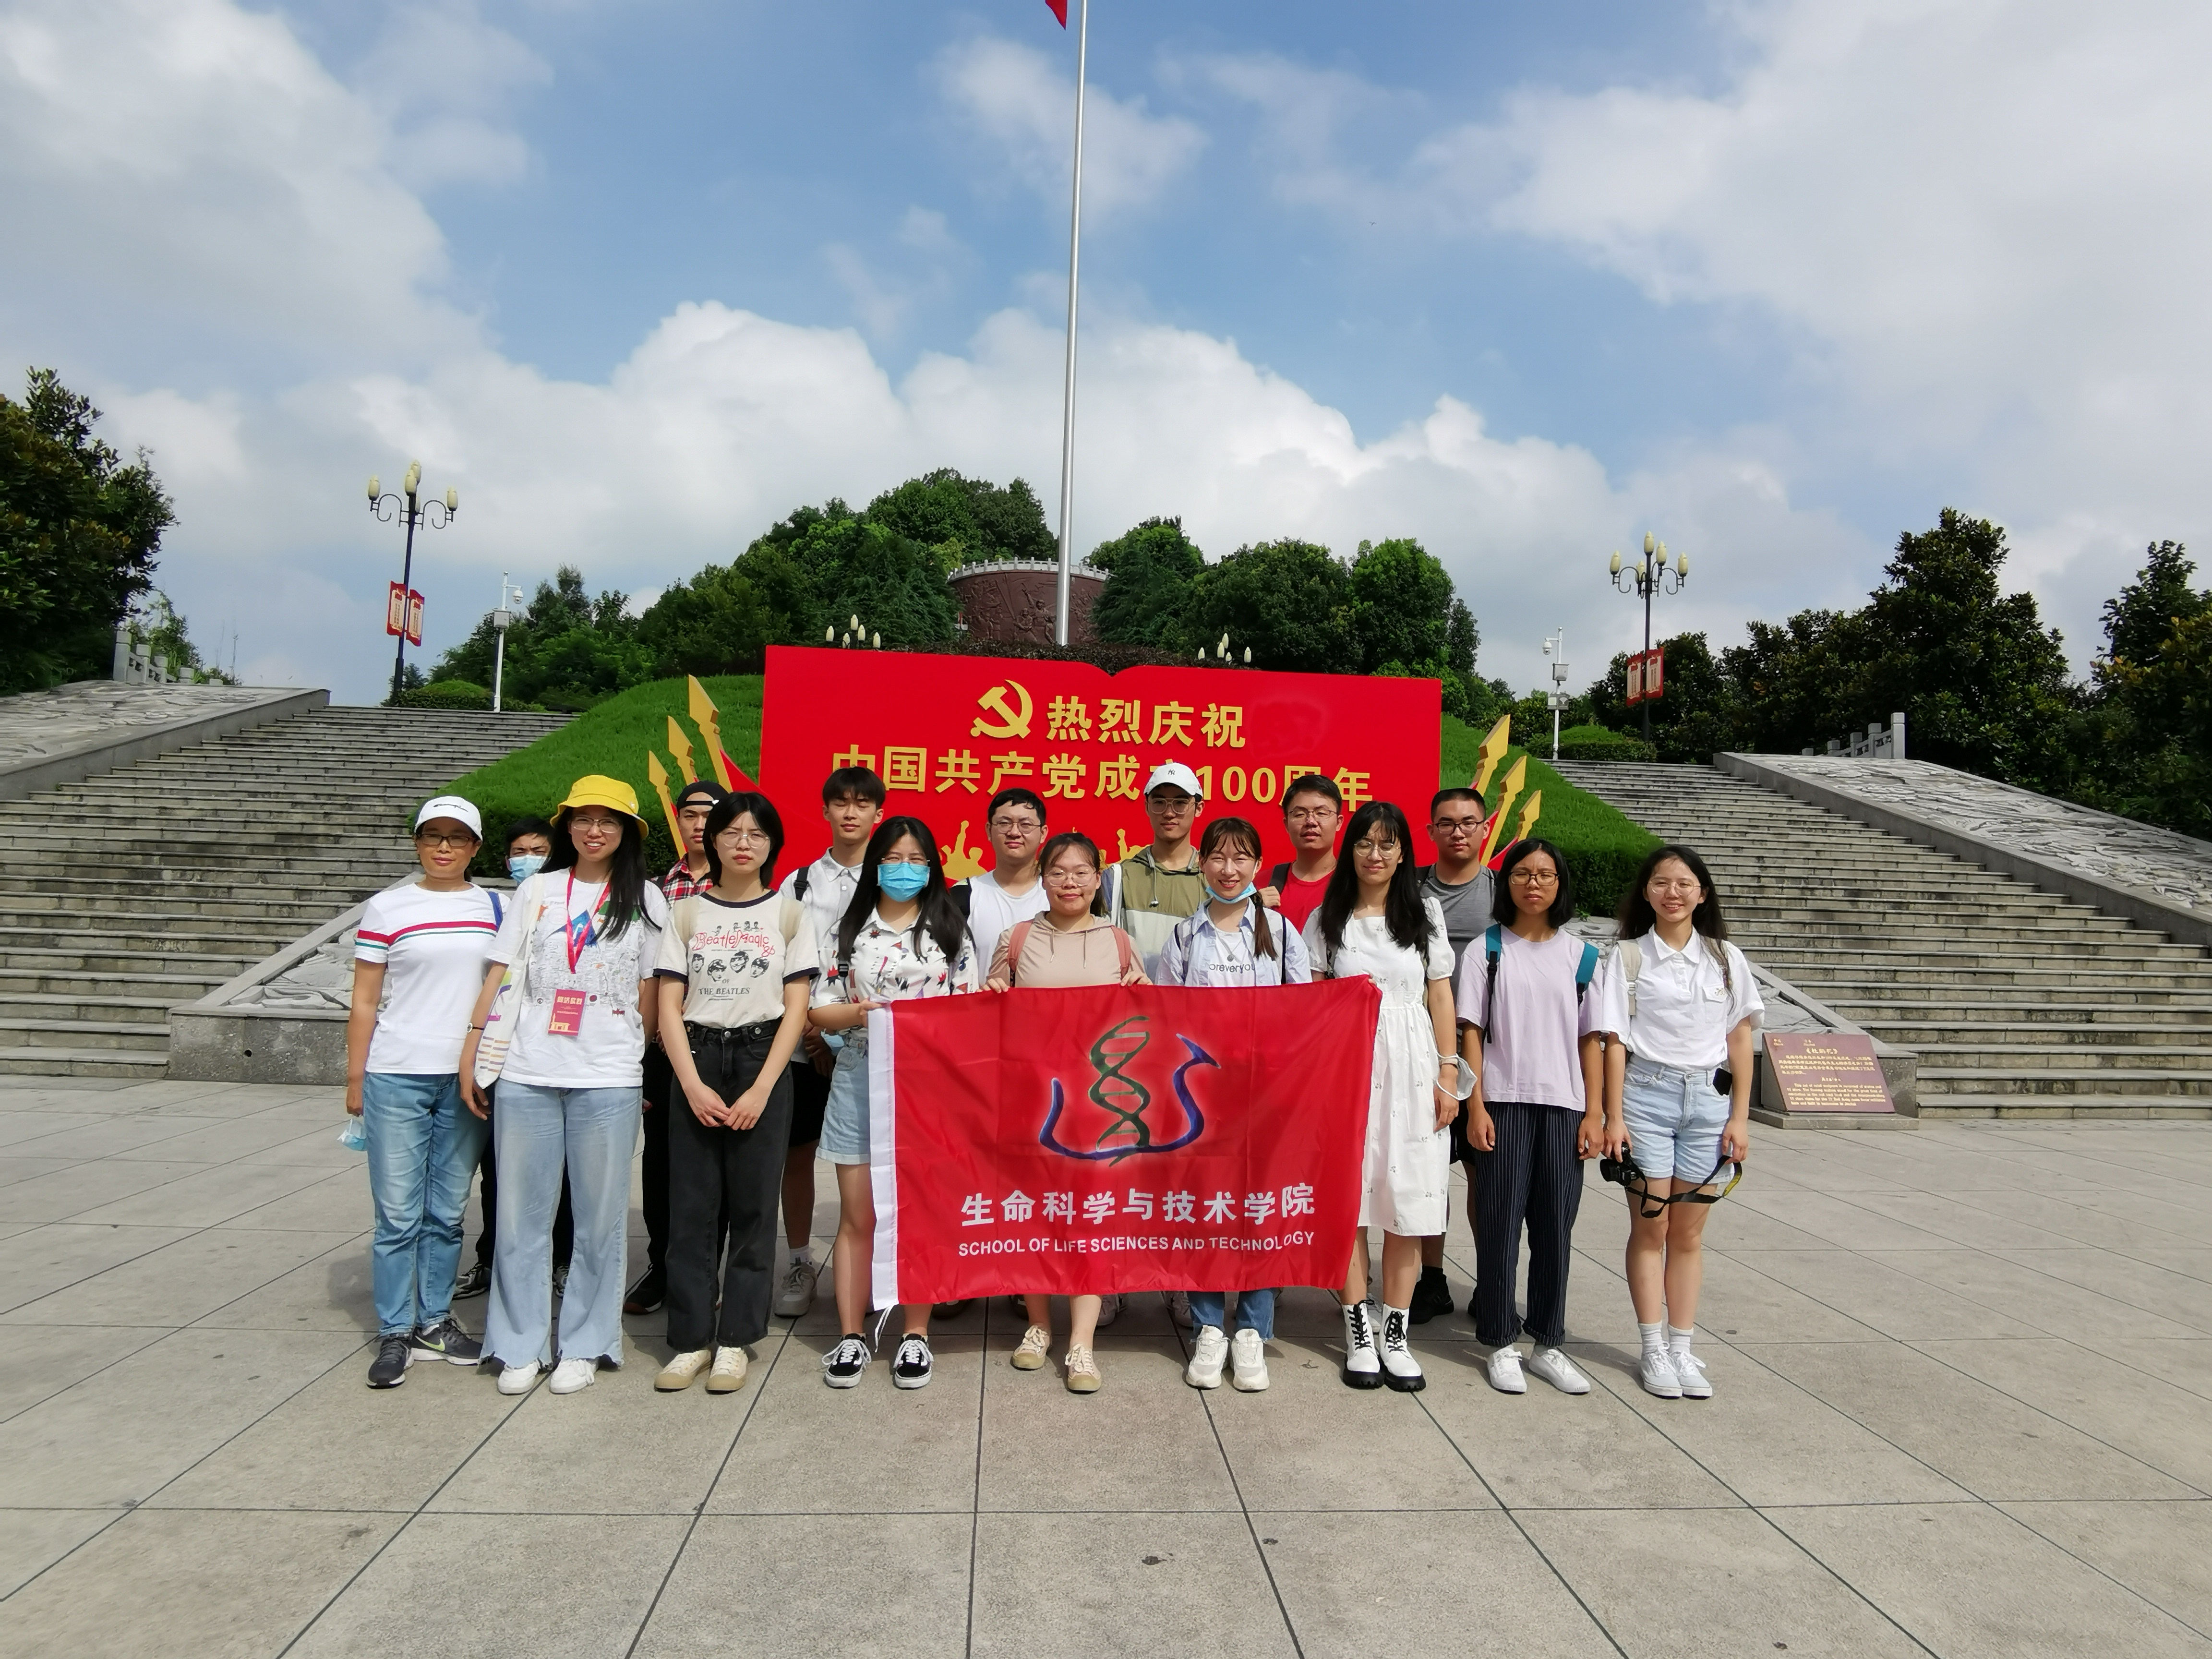
\includegraphics[width=0.7\textwidth]{image/WechatIMG110.jpeg}
    \caption{指导老师及全体实习人员}
    \label{STAFF1}
\end{figure}
\section*{致谢} 

笔者对接待单位及接待单位的经理,主管及员工,表示由衷的感谢:他们的精心安排与细心指导,是本次实习能够顺利完成,是本次实习能够让大家都有所收获的必不可缺的条件。

也感谢本次实习的带队老师对实习的统筹与对同学的指导,老师对与同学学习、食宿的关照,也是实习能完成对重要组成部分。

此外,还需要感谢同行的同学们,同学们在讨论中的见解使得笔者受益良多。

\begin{figure}[H]
    \centering
    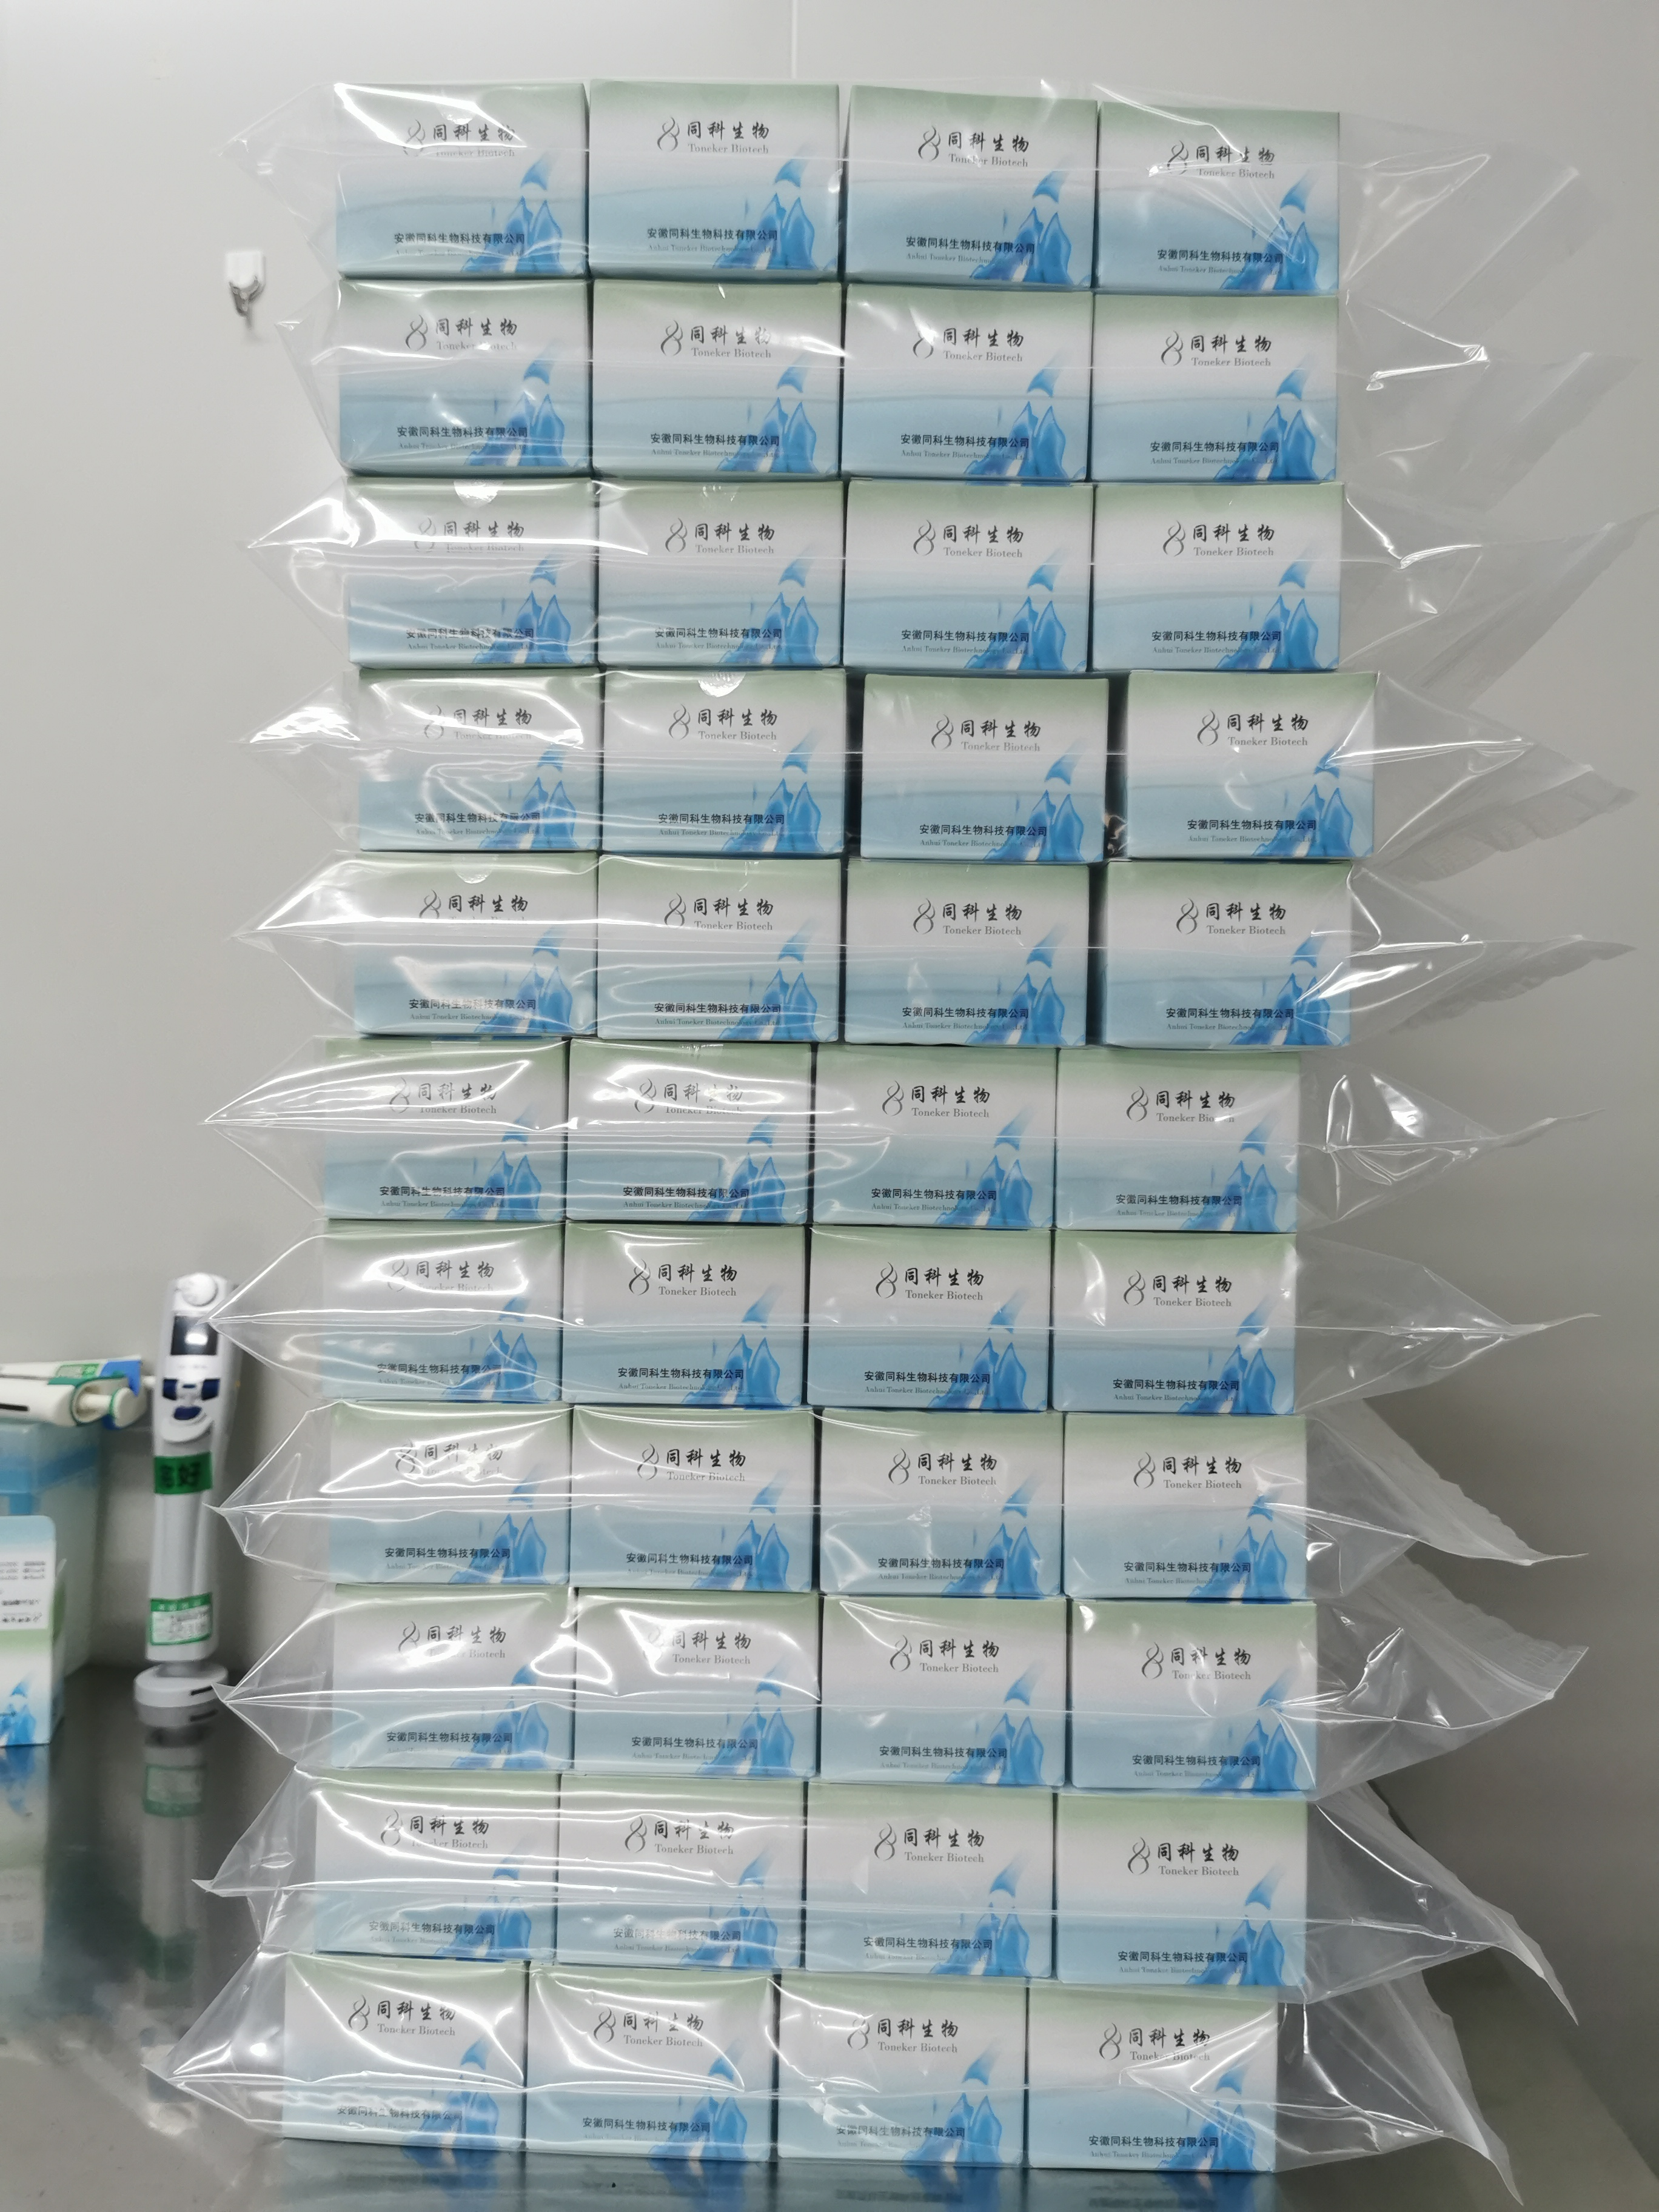
\includegraphics[width=0.7\textwidth]{image/WechatIMG92.jpeg}
    \caption{本次实习生产的部分产品成品}
    \label{STAFF2}
\end{figure}

\end{document}
